%%%%%%%%%%%%%%%%%%%%%%%%%%%%%%%%%%%%%%%%%%%%%%%%%%%%%%%%%%%%%%%%%%%%%%%%%%%%%%%%
%2345678901234567890123456789012345678901234567890123456789012345678901234567890
%        1         2         3         4         5         6         7         8

\documentclass[letterpaper, 10 pt, conference]{ieeeconf}  % Comment this line out if you need a4paper

%\documentclass[a4paper, 10pt, conference]{ieeeconf}      % Use this line for a4 paper

\IEEEoverridecommandlockouts                              % This command is only needed if 
                                                          % you want to use the \thanks command

\overrideIEEEmargins                                      % Needed to meet printer requirements.

% See the \addtolength command later in the file to balance the column lengths
% on the last page of the document

% The following packages can be found on http:\\www.ctan.org
\usepackage{graphics} % for pdf, bitmapped graphics files
\usepackage{epsfig} % for postscript graphics files
\usepackage{mathptmx} % assumes new font selection scheme installed
\usepackage{times} % assumes new font selection scheme installed
\usepackage{amsmath} % assumes amsmath package installed
\usepackage{amssymb}  % assumes amsmath package installed
\usepackage{float}
\usepackage{graphicx}% http://ctan.org/pkg/graphicx

\title{\LARGE \bf
ESE650 Project 2: Orientation Estimation
}


\author{Achille Verheye% <-this % stops a space
}


\begin{document}



\maketitle
\thispagestyle{empty}
\pagestyle{empty}


%%%%%%%%%%%%%%%%%%%%%%%%%%%%%%%%%%%%%%%%%%%%%%%%%%%%%%%%%%%%%%%%%%%%%%%%%%%%%%%%
\begin{abstract}

This report describes the methods used and decisions made for Project 2 for the class ESE650 Learning in Robotics at the University of Pennsylvania. An Unscented Kalman Filter was used in quaternion representation to fuse and filter data from an accelerometer and a gyroscope. The underlying state aimed to estimate the underlying orientation the Inertial Measurement Unit achieved. Attached to the IMU was a camera which took sequential pictures during rotation. Filtered orientation was then used to stitch these images together to create a panorama of the environment.

\end{abstract}


%%%%%%%%%%%%%%%%%%%%%%%%%%%%%%%%%%%%%%%%%%%%%%%%%%%%%%%%%%%%%%%%%%%%%%%%%%%%%%%%
\section{INTRODUCTION}
Sensor fusion and filtering is a common problem in robotics and many other domains. Sensors measure an effect of an underlying state, in this report orientation, and sometimes the absolute state directly. The data is oftentimes noisy and contradicts other sensory information. In many cases, one set of sensors relates to the underlying state incrementally and fairly accurate but drifts over time due to small error accumulation while another set of sensors measures an absolute value that relates to the underlying state directly but is very noisy. The Kalman Filter has been proven to work well in these cases, using the incremental update in a prediction step and correcting using the absolute, noisy data in an update step.

\section{PROBLEM FORMULATION}
A device consisting of an Inertial Measurement Unit (IMU) and a fixed camera aligned with the IMU at a fixed distance is rotated in the world frame. The device is pictured in Figure \ref{device}. The IMU records acceleration and angular velocities along three dimensions at consecutive timesteps. Concurrently, the camera records images from its point of view at certain timesteps. The goal is to fuse acceleration and gyroscopic data from the IMU to estimate the underlying orientation at each timestep. This orientation is then used to stitch the images taken by the camera together into a panoramic image.

   \begin{figure}[thpb]
      \centering
      \framebox{\parbox{3in}{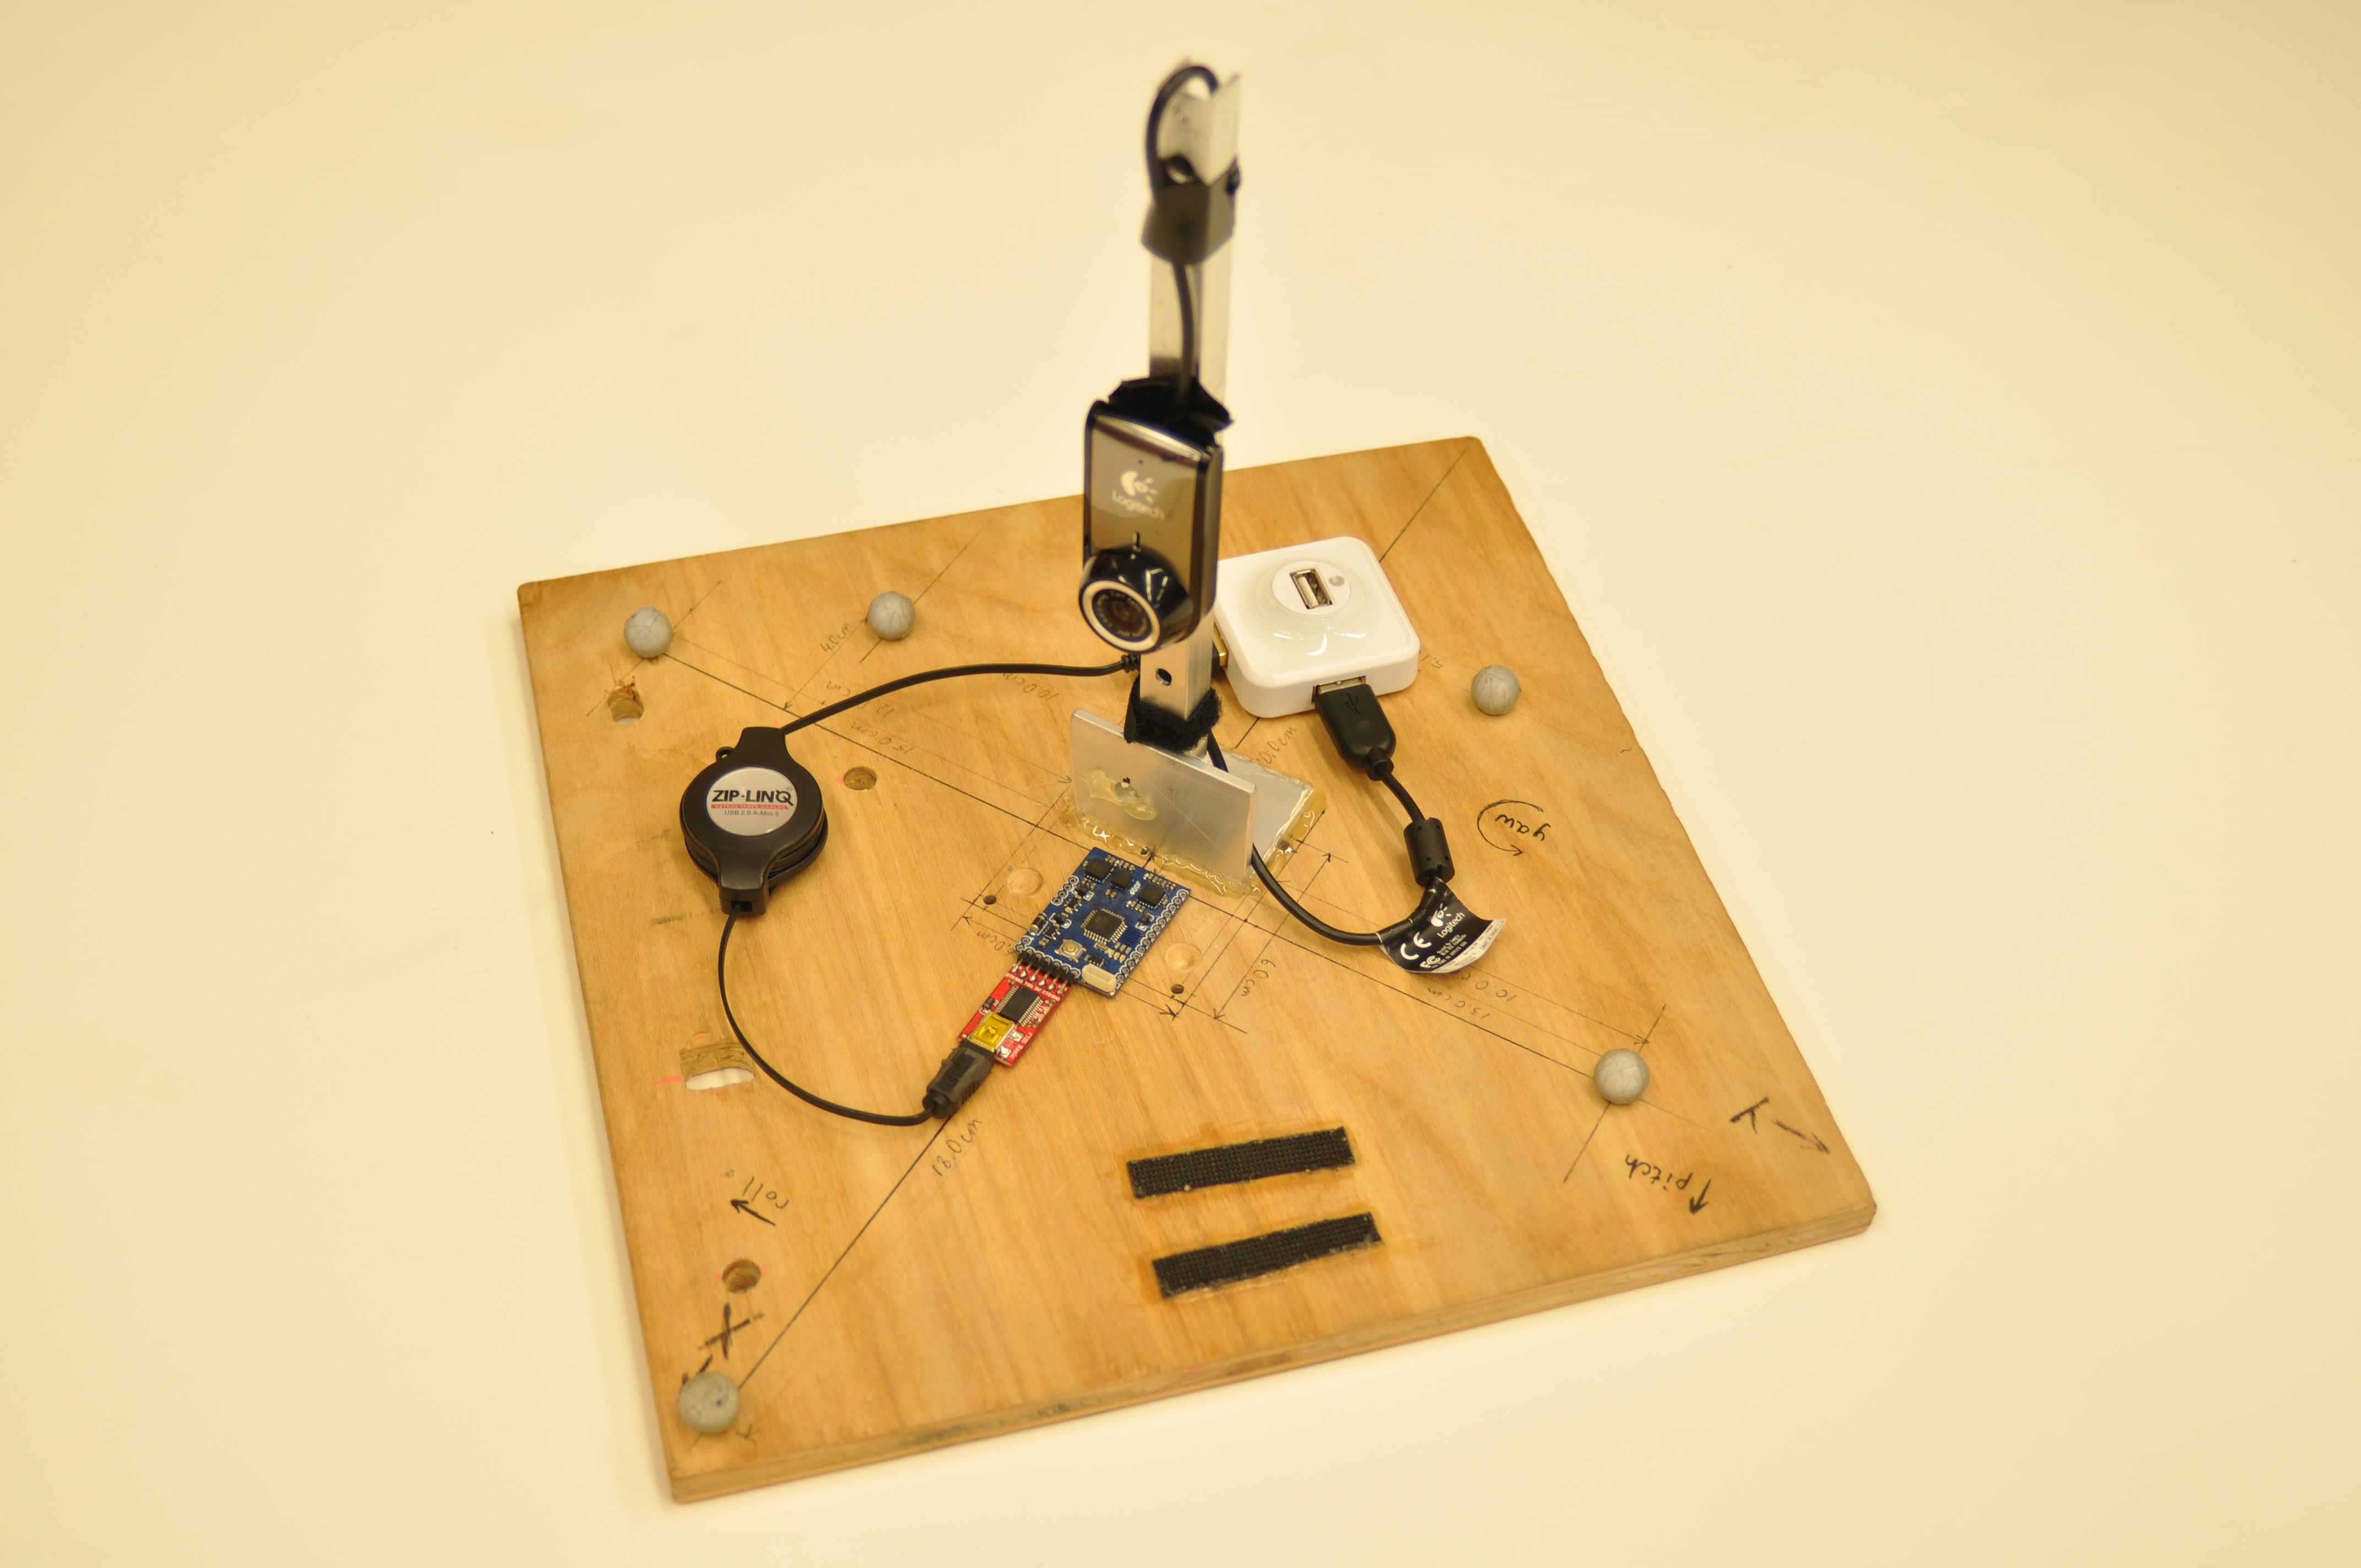
\includegraphics[scale=0.21]{proj2_platform1.jpg}}}
      \caption{Device used to capture images and data from an IMU.}
      \label{device}
   \end{figure}

When considering rotations, a minimal representation that does not suffer from gimbal lock is the quaternion. The quaternion can be converted from and to the axis/angle representation easily and represents rotations using only four numbers as opposed to nine using rotation matrices in SO(3).
$$q_{\theta, n} = \left(cos\left(\frac{\theta}{2}\right), n_x sin\left(\frac{\theta}{2}\right), n_y sin\left(\frac{\theta}{2}\right), n_z sin\left(\frac{\theta}{2}\right)\right)$$
However, applying these quaternions as rotations is inherently nonlinear. This violates the assumption of linearity used in the classical Kalman Filter. Two approaches exist to accomodate this nonlinearity. One is to approximate (linearize) the equations which allows for calculation of the parameters for a Gaussian distribution explicitly. This has proven to not be effective for very nonlinear process models. Another option is to sample points of the Gaussian distribution, called sigma points, feed them through the nonlinear process model, and approximate the resulting (nonlinear) distribution with a new Gaussian. This  Unscented Kalman Filter (UKF) proves to work much better in this case. It is explained for this case in Section \ref{sigma}.


\section{TECHNICAL APPROACH}

\subsection{Two Options for implementation}
Two options exist for executing the UKF, both based on the implementation as described in Kraft \cite{c1}. The options differ in selection of inputs and state, but should both include the orientation quaternion and yield the same results given the same parameters and data. The Kalman Filter consists of a prediction step, corresponding to using the process model to extrapolate the predicted next step based on the current state and input, and an update step. The prediction then relates to the expected output via the observation model. The update step relates the measurement in the next step to this expected output and optimally adjusts internal parameters (gain $K_k$) to improve filtering in the next iteration. The estimate is also adjusted based on the measurement data and the gain.

\subsubsection{Option 1: Angular velocity in state}
This option most closely follows the approach by Kraft. The state $x_t$ is seven dimensional consisting of a quaternion (4D) and an angular velocity vector (3D) vector. The process model relates two consecutive states and is as follows:
$$
\begin{pmatrix}
q_{t+1} \\
\omega_{t+1}
\end{pmatrix}
=
\begin{pmatrix}
q_t q_{noise} q_{\Delta} \\
\omega_t + noise_t
\end{pmatrix}
$$
Where the multiplication $q_t q_{noise} q_{\Delta}$ is a quaternion multiplication, a nonlinear operation that is different from regular multiplication. $q_t$ is the previous state orientation. $q_{\Delta}$ transforms the state to the predicted new state based on the angular velocity of the previous state ($\omega_t$). Gaussian noise is added in this step and acts as regularization to improve robustness. 

The predicted state for the next step is then fed through the observation model. This model relates orientation to the acceleration vector expected in the orientation at that time. As the normal force due to gravitation points along the z-axis of the IMU, the resulting vector g' will be rotated as dictated by the orientation. 
$$
\begin{pmatrix}
z_{acc} \\
z_{\omega}
\end{pmatrix}
=
\begin{pmatrix}
q_t^{-1} g q_t \\
\omega_t + noise_t
\end{pmatrix}
$$

This observation result can then be compared to the actual measured values in the next step to produce an innovation. This innovation, pre-multiplied by the Kalman gain, then determines the filtered estimate of the state and is used for the next iteration of filtering. The details of computing the gain can be found in Kraft \cite{c1} and in Section \ref{sigma} and \ref{other}.

\subsubsection{Option 2: Angular velocity as input}
A perhaps more intuitive way, with direct parallels to filtering in cars using dead reckoning and GPS data is to use gyroscopic data as an input to the process model and to only include the orientation in the state. The output of the observation model for the predicted state is then compared to the measurement of the acceleration from the IMU. This approach also reduces the size of correlation matrices and vectors making debugging easier, is less prone to human error and makes code shorter and easier to understand. From this point, this option is used, but all considerations and calculations apply to Option 1 as well.

\subsection{Sigma Points} \label{sigma}
The Unscented Kalman Filter makes use of sigma points to represent a distribution that is passed through a nonlinear model. These points are then used to approximate the resulting complex distribution with a Gaussian distribution. This is illustrated in Figure \ref{distribution}.
   \begin{figure}[thpb]
      \centering
      \framebox{\parbox{3in}{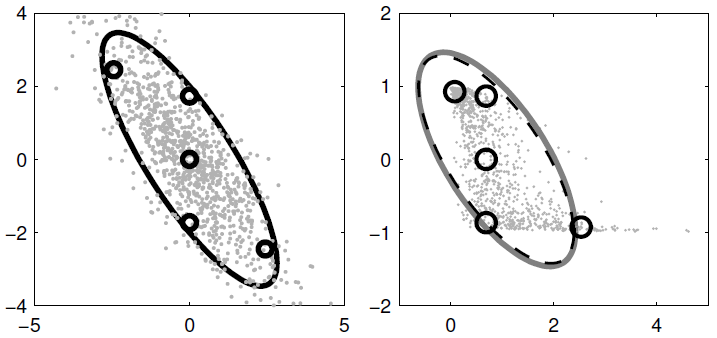
\includegraphics[scale=0.5]{distribution-illustration}}}
      
      \caption{transformation from the sigma points (left) through the process model, yielding a nonlinear distribution, approximated by a Gaussian (right).}
      \label{distribution}
   \end{figure}

The mean and covariance form a better representation of the state distribution than the Extended Kalman Filter would. These points can also be used to calculate expected outputs by feeding them through the observation model. However, the sigma points became skewed by the process model, so to improve performance  we can find new sigma points that have the same mean and covariance as the previous points.

It must be noted that determining mean and covariance of sigma points is not trivial due to the quaternion representation. The sigma points can be found as the square root of the covariance of the previous state estimate. The noise can easily be added in this step as in the form of a noise covariance. The $n$ columns of the resulting matrix are then multiplied by a constant scaling factor $\pm \sqrt{2n}$ which leads to $2n$ columns centered around zero. The sigma points, representing states, are then converted to quaternion format using the exponential operator and are rotated using the state estimate of the previous iteration. That state was also added as a sigma points, yielding $2n+1$ sigma points.

The mean of a set of quaternions is especially tricky as the barycentric mean doesn't yield the actual mean rotation quaternion due to the periodic aspect of rotations. Therefore, an iterative gradient descent algorithm was used to calculate the mean value of the sigma points. As it turns out, a side product, the error vector, of that calculation is useful later in the calculation of the covariance of the sigma points. That error vector consists of $2n+1$ that each correspond to a sigma point. Applying the quaternion format of these error vectors to the average quaternion yields the corresponding sigma points.

The covariance of the sigma points, the a priori state vector covariance $P_k^-$ is used to update the a posteriori covariance $P_k$, which becomes the basis for the next iteration. It is calculated from the error vectors, which makes sense as they describe how far each angle is away from the mean. Each sigma point adds to $P_k^-$ by the outer product of this error vector with itself. The set of error vectors, $W_i$, is stored as it can be used in the calculation of the cross-correlation matrix $P_{xz}$

In both the calculation of the mean as well as the covariance as described above, other than in the paper by Kraft, weights are used to emphasize the relative importance of the previous state estimate while also normalizing. A quaternion that is related to a higher weight will pull the average quaternion towards its value. 

\subsection{Other Considerations} \label{other}
The measurements from the IMU have to be scaled and shifted to account for the bias, coordinate system, and units of the angular velocity and acceleration. These scaling factors can be found from the data sheet for the IMU. Instead of using the bias provided by the data sheet, the sensor was calibrated based on the first values the gyroscope and accelerometer recorded. The assumption made is that the device is stationary during the first seconds of recording (angular velocity components zero and acceleration in x and y zero, acceleration due to gravity equal to one). Alternatively, the first several values could be averaged to avoid errors at the start, but it was experimentally determined that the effect of this change was negligible. In any case, a user should understand the incoming values as to make sure these assumptions are asserted.

The noise covariance matrix $Q$ for the process model and $R$ for the observation model were found experimentally by comparing filter results to vicon ground truth orientation. $Q$ was set to $10^{-4}$ while $R$ yielded optimal results at a value  of $6*10^{-3}$. Setting $Q$ too high introduces error in the prediction step, yielding random noise in the overall result. Setting $R$ very high makes the update step put little 'trust' in the accelerometer data, yielding a filter for which the results are close to that of the prediction step alone. An idea was to relate this noise to the difference in time $\Delta_t$ between each consecutive timestep, but that turned out to have very little effect on the end result.

Special attention has to be paid to the several conversion from rotation vectors to quaternions and to order of multiplication, which was not always clear from Kraft. Small mistakes yielded large errors and a lot of testing had to be done to ensure that the results were optimal. In fact, it is hard to know how close the filter values should be to the ground truth to make the result satifsying. Judging from the panoramas made (Section \ref{panosection}), small errors had a rather large impact on the result, but it is unlikely that it is possible to match the ground truth values exactly with a filter.

\subsection{Panoramic Stitching} \label{panosection}
Since the camera was aligned with the body frame of the capturing device and thus the IMU, the filtered orientation allowed for simple stitching of the sequential images into a single panoramic image. By transforming and projecting the images sequentially, an animation of the stitching process was made, providing a good visualization of the rotations the device underwent. Results of this process can be seen in Figures \ref{overwrite} - \ref{notoverwrite}.

Construction of the panorama was achieved in multiple steps in an easy to follow object oriented fashion. The panorama object requires four parameters: the images captured by the camera, the timestamps of these images, a set of orientations, and the timestamps corresponding to each orientation. The high-level process is as follows. First, images are matched to the closest filtered orientation in time using the two sets of time stamps. Not all orientations are used as there are more images than orientations. An incoming image is treated as spherical around the device at a fixed distance. The first steps of the process are the same for all images, therefore a 'coordinate image' is made that is used for all images. This matrix contains the coordinates of each pixel. It is first shifted so the middle of the image corresponds to the origin and the axes align with that of the capturing device. Scaling of the image ensures that the image has a field of view in horizontal direction of 60 degrees and 45 degrees in vertical direction. The pixels now represent a longitude and latitude on the unit sphere with center in the origin of the camera.
\begin{align*}
x &= r \cos(latitude) \cos(longitude) \\
y &= r \cos(latitude) \sin(longitude) \\
z &= r \sin(latitude)
\end{align*}
Instead of representing this coordinate matrix in the same shape as the incoming image, it is unrolled into a 3 by N matrix as to allow vectorized computation of transformation. Particularly, in the next step the rotation matrix is used to rotate the coordinate locations to the new location on the sphere with a single operation. This concludes the matching of the orientations with the images.
The next step is to project these images, represented by 3D cartesian coordinates on a 2D panoramic image. To do this, the images are first transformed back to spherical space, are then mapped to cylindrical space, and finally the cylinder is 'unwrapped' to create a panorama.
\begin{equation}
\begin{aligned}
latitude &= \arctan2\left(z, \sqrt{x^2 + y^2}\right) \\
longitude &= \arctan2\left(y, x\right) \\
r &= 1
\label{cart2spher}
\end{aligned}
\end{equation}

Equations \ref{cart2spher} convert cartesian coordinates into spherical, while Equations \ref{spher2cyl} convert these spherical coordinates into cylindrical coordinates, which allows for easy unwrapping onto a panorama.

\begin{equation}
\begin{aligned}height &= \tan(latitude) \\
longitude &= longitude \\
r &= 1
\label{spher2cyl}
\end{aligned}
\end{equation}

Since the panorama size is only two-dimensional and has limited size, pixels pointing upward and downward in the coordinate frame must be cut off or scaled in the conversion from spherical to cylindrical coordinates. This is done by clipping all resulting values outside a range of $\pm \pi$.

In the final step, the cylinder is unwrapped by simply converting the longitude and height of the cylinder to pixels so that the range of orientations is distributed over the size of the panorama appropriately. Mapping also has to include shifting the locations as the panoramic image has its coordinate system in the top left of the image. The panorama image can then be indexed in each step after casting the arrays to integer format with a single operation, placing the new image in the panorama.

Two options were explored in this last step. One was to overwrite previously assigned pixels while the other was to keep the original pixel in place and only update unseen locations. Results using the vicon ground truth orientation are in Figures \ref{overwrite} and \ref{notoverwrite}. As can be seen, differences are minimal. The choice of the option to use depends on the use case. Overwriting yields smoother transitions in the video but due to inaccuracies in the filter and orientation data accumulating over time, the result tends to be slightly shifted compared to the physical world. However, this methodology can easily be extended and provides a basis for more advanced stitching techniques to ensure smooth transitions.

\begin{figure*} [ht]
  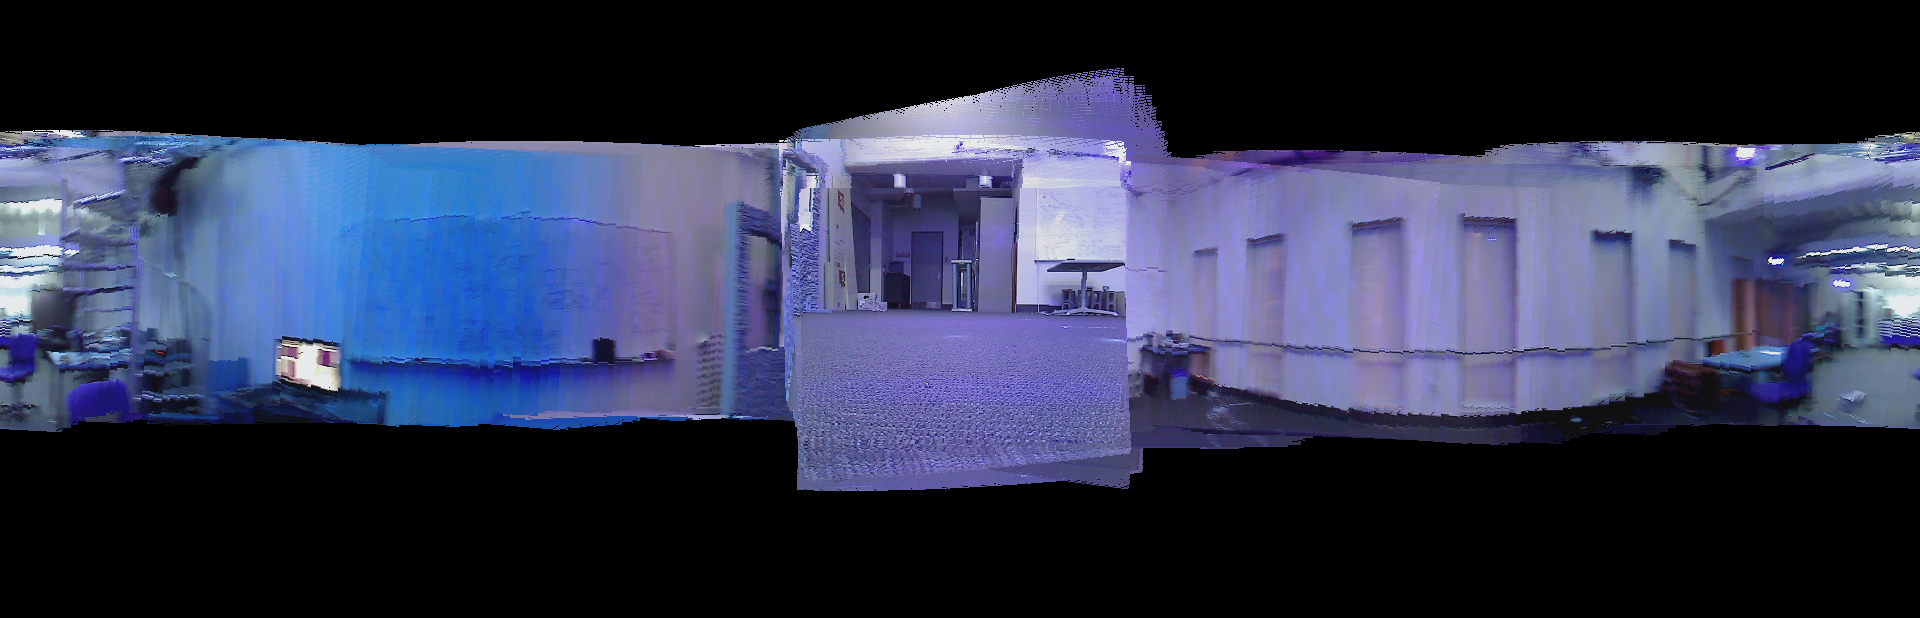
\includegraphics[width=\textwidth,height=5cm]{panorama_vicon_8_crop}
  \caption{Panoramic image constructed from Vicon ground truth set 8 using overwriting.}
  \label{overwrite}
\end{figure*}

\begin{figure*} [ht]
  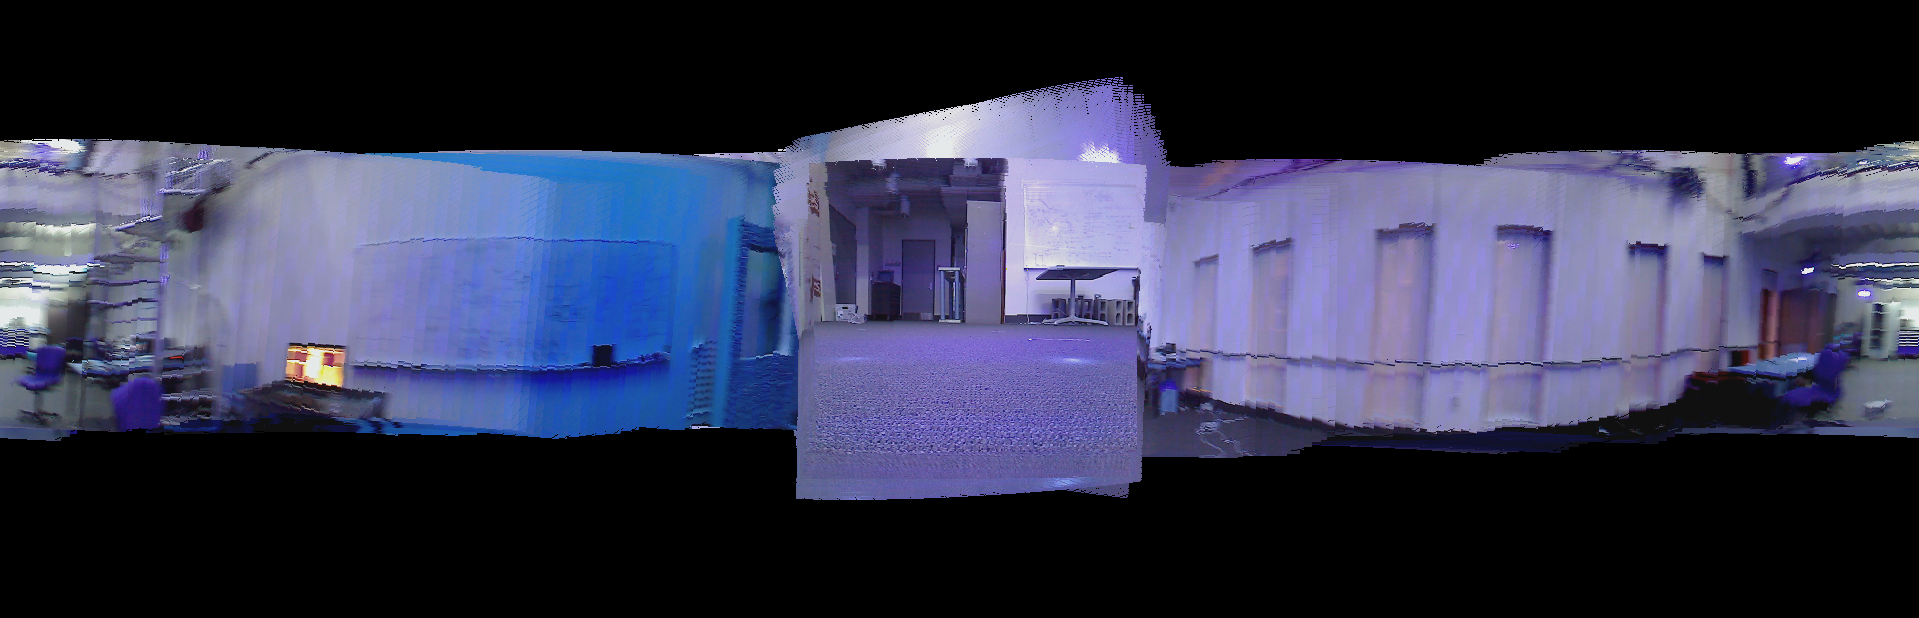
\includegraphics[width=\textwidth,height=5cm]{panorama_vicon_8_no_overwrite}
  \caption{Panoramic image constructed from Vicon ground truth set 8 not overwriting.}
  \label{notoverwrite}
\end{figure*}


\section{RESULTS}

Figures \ref{compare1} to \ref{compare9} show results using the prediction step and for the complete filter compared to the vicon ground truth. For data set 1, drifting of the orientation later in the recording is corrected by the acceleration update. Since the accelerometer cannot pick up yaw when the z-axis is aligned with the gravity vector, a small error is introduced by the update towards the end. The update does negatively influence the second peak in the roll and the yaw. These were resolved by calibrating the noise covariance matrices but changing these noises worsened results for other data sets. Data set 2's prediction is already of fairly bad quality, and even the update step can not correct all of the error. Performance is much better using the full UKF though. The UKF does a good job of bringing the orientation estimates closer to the ground truth but still deviates with an absolute value of about $\pm 0.2 rad$ in some cases. Since camera data is not available for this data set, it is hard to verify where the problem exactly comes from and if significant improvement can be made. Data set 4 is the only set that resulted in significant error, mainly in the yaw component. This might be due to the fact that the reset pin fired during recording. Estimation in data set 5 is greatly improved by the update with some relatively small errors in roll and pitch. Due to the fact that these angles wrap around, the yaw shows that the angles are $2\pi$ off, which results in the same orientation. Filtering performed on data set 6 yielded the best results of all sets. Prediction using just the gyroscope already yielded very accurate results, especially for the yaw. The pitch did benefit from the innovation introduced by the measurement update, shifting the graph down, almost exactly matching the ground truth. Data set 7 yielded similar results as data set 6, with just minor discrepancies in the yaw component. Data set 8 was shaky and thus noisy. Prediction yielded good results but needed calibration by the update step. The power of the update step is especially apparent in the improvement of the pitch and roll, pulling the tail almost completely back to ground. Finally, data set 9 as in Figure \ref{compare9} suffers from very bad prediction. The update step makes a significant improvement, but the truth still deviates at some points in time. 

Figure \ref{panorama8} shows the panorama generated using filtered data. As can be seen, small deviations from the actual orientation result in larger deviations in the panorama. This is also due to the fact that the stitching is purely based on rotation and not on translation of the device. We can see this from the ground truth panorama in Figure \ref{overwrite}. When the device is lifted off the ground and placed back, no change in rotation occurs, but the image slighly shifts with each movement. Advanced image stitching using vectors and contour mapping again can improve the result here.

Processing and plotting of the entire list of IMU measurements ($\pm 3500$) measurements using the UKF took about 15 seconds on average to complete.

   
\begin{figure*} [ht]
  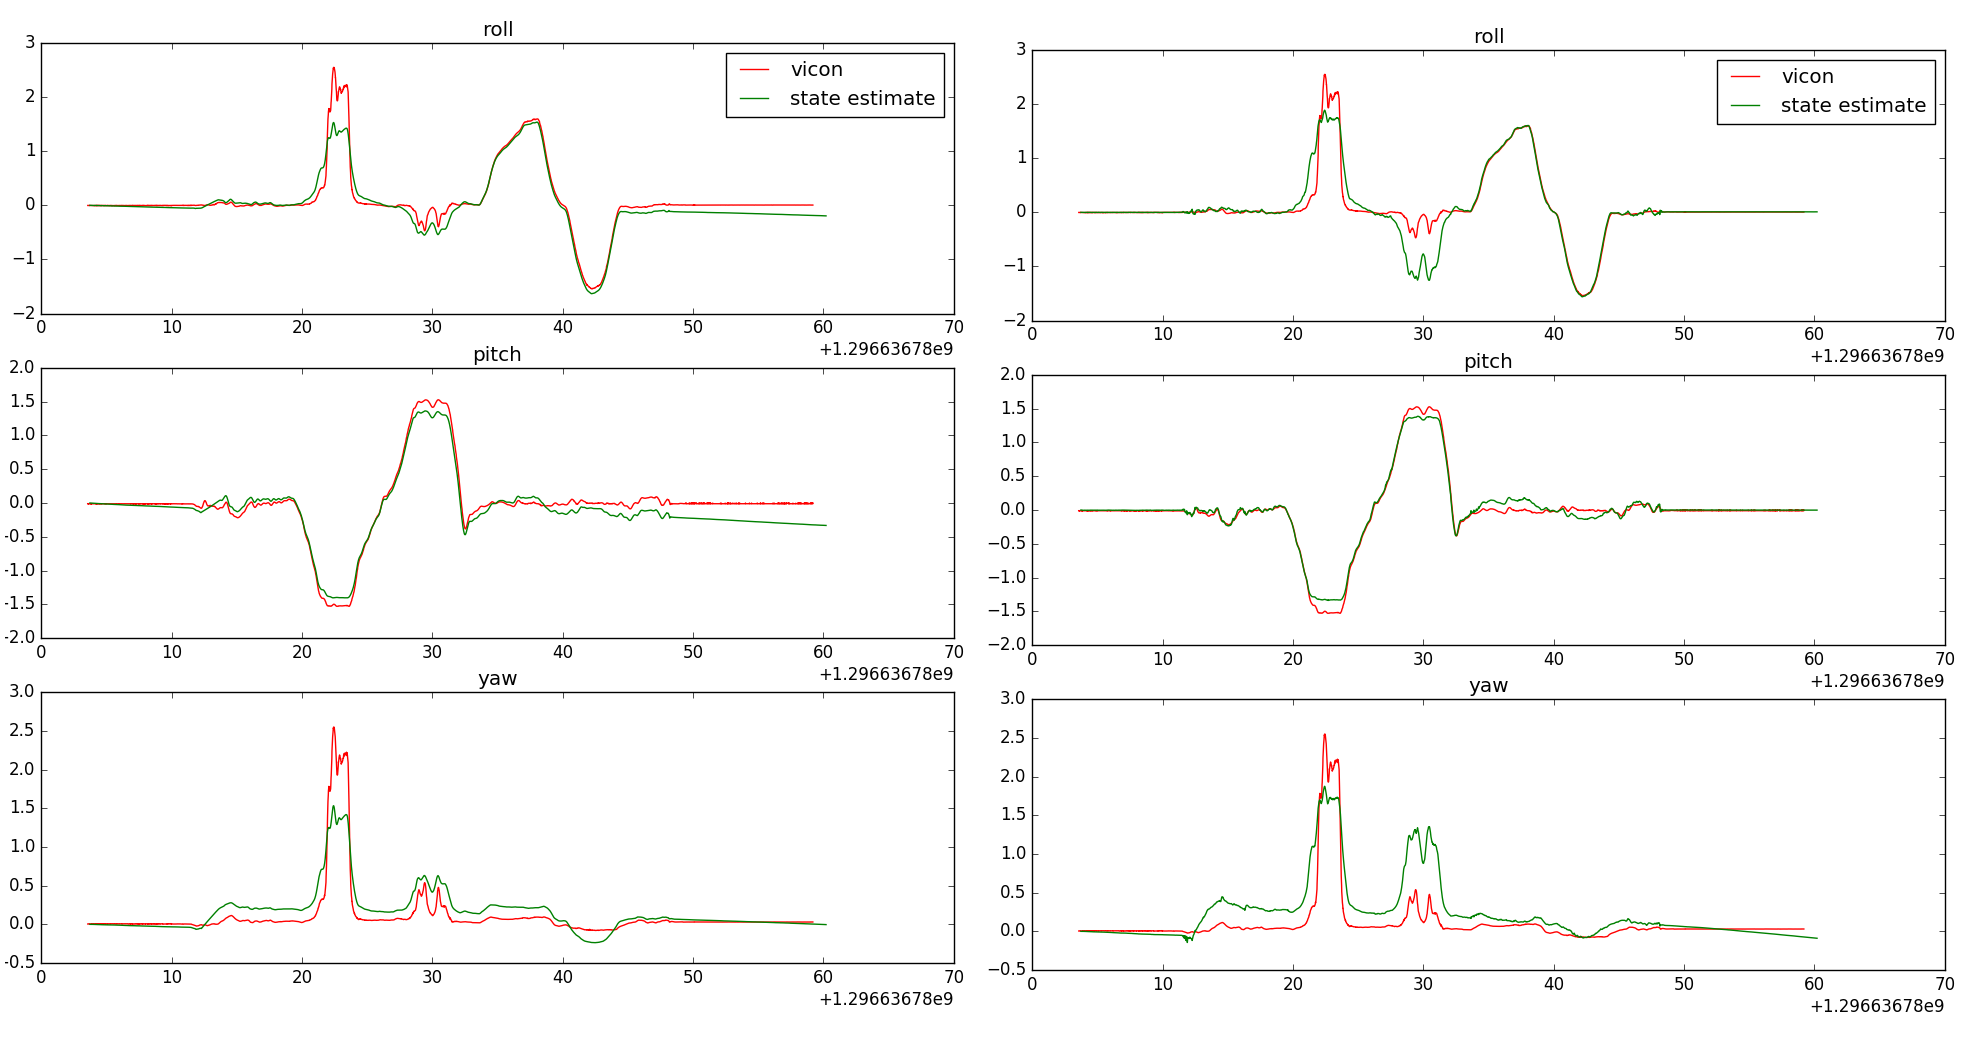
\includegraphics[width=\textwidth,height=5cm]{compare1}
  \caption{Left: Prediction only. Right: UKF compared to ground truth (red) (data set 1).}
  \label{compare1}
\end{figure*}   
 
\begin{figure*} [ht]
  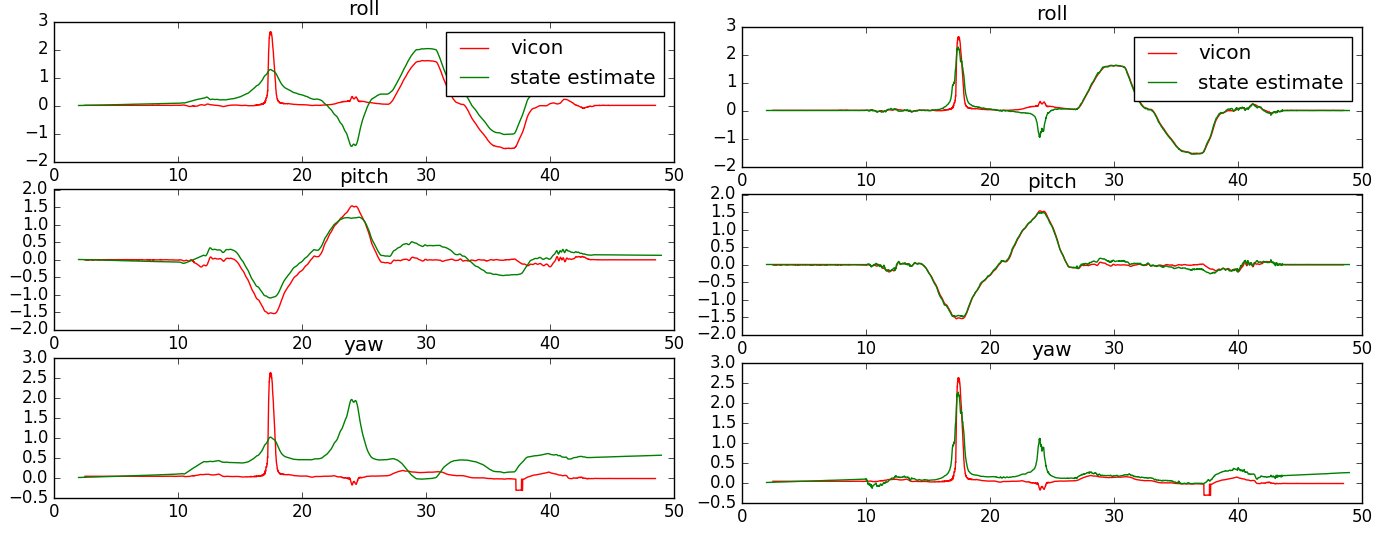
\includegraphics[width=\textwidth,height=5cm]{compare2}
  \caption{Left: Prediction only. Right: UKF compared to ground truth (red) (data set 2).}
  \label{compare2}
\end{figure*} 

\begin{figure*}
  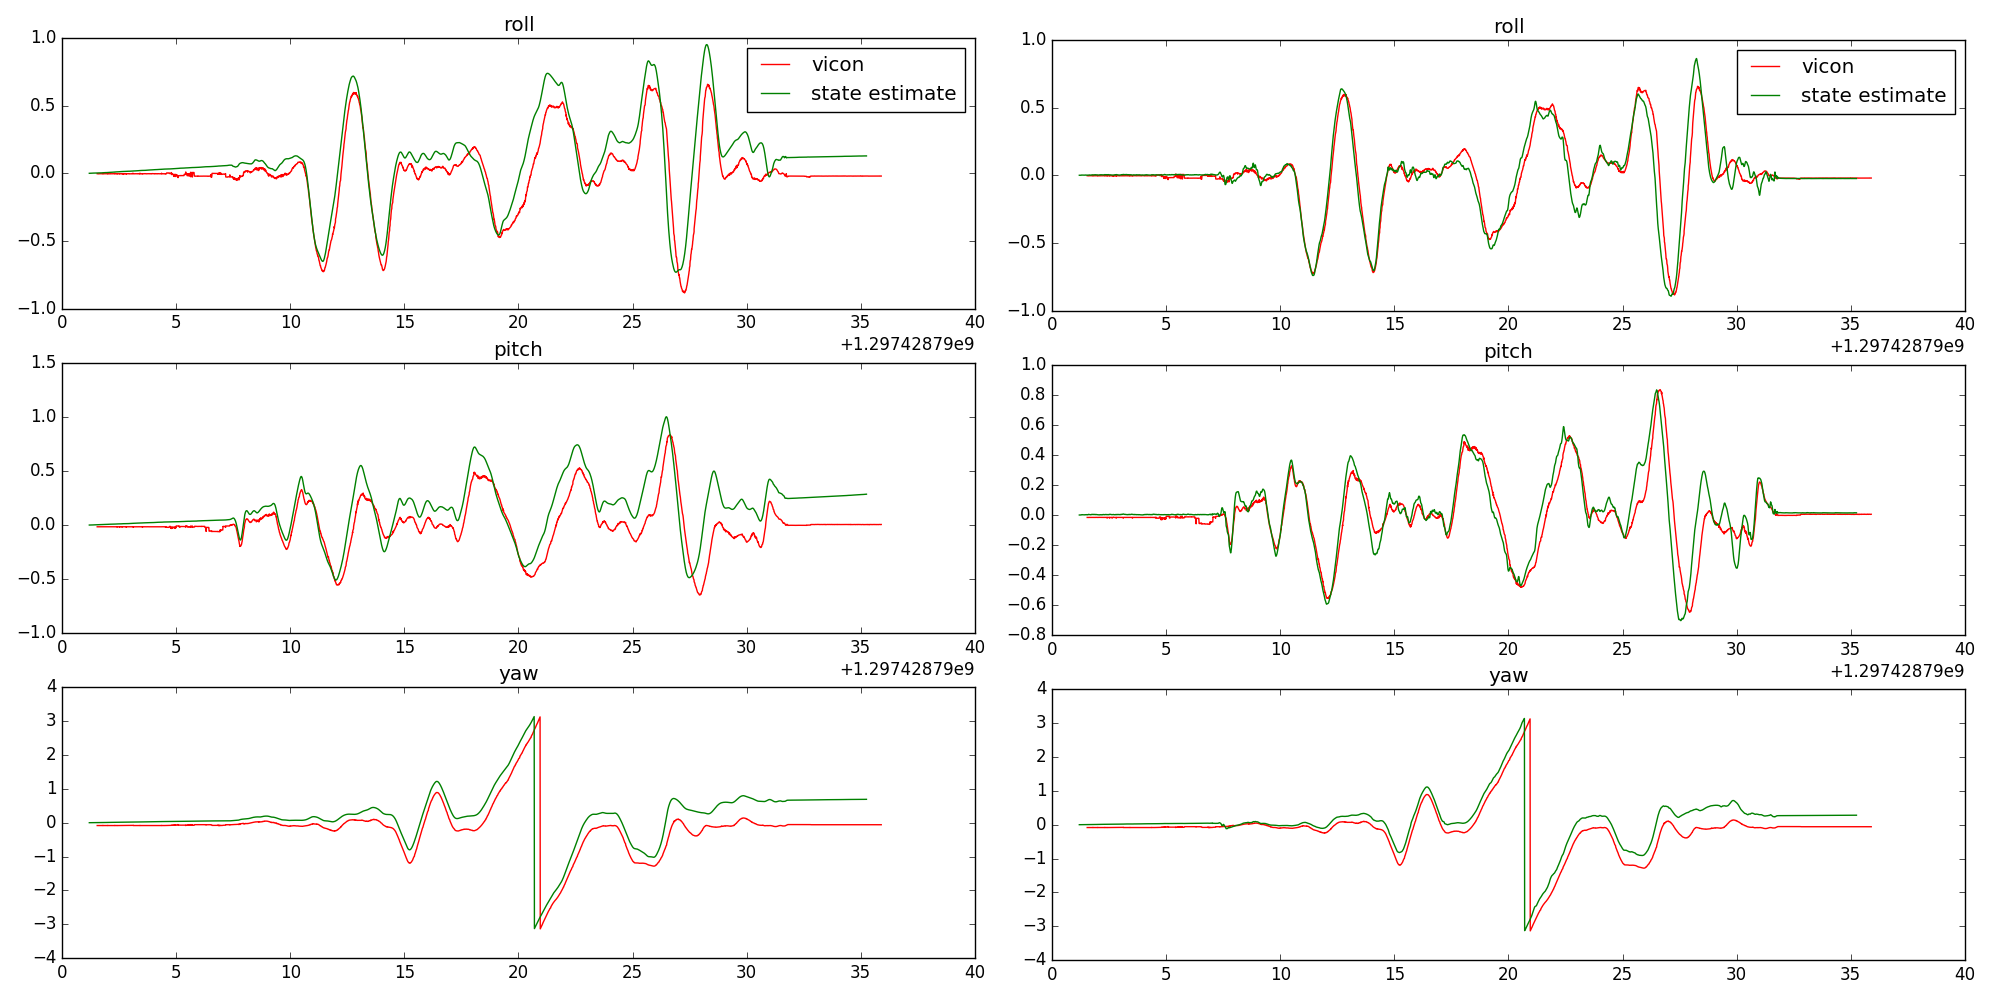
\includegraphics[width=\textwidth,height=5cm]{compare3}
  \caption{Left: Prediction only. Right: UKF compared to ground truth (red) (data set 3).}
  \label{compare3}
\end{figure*} 

\begin{figure*}
  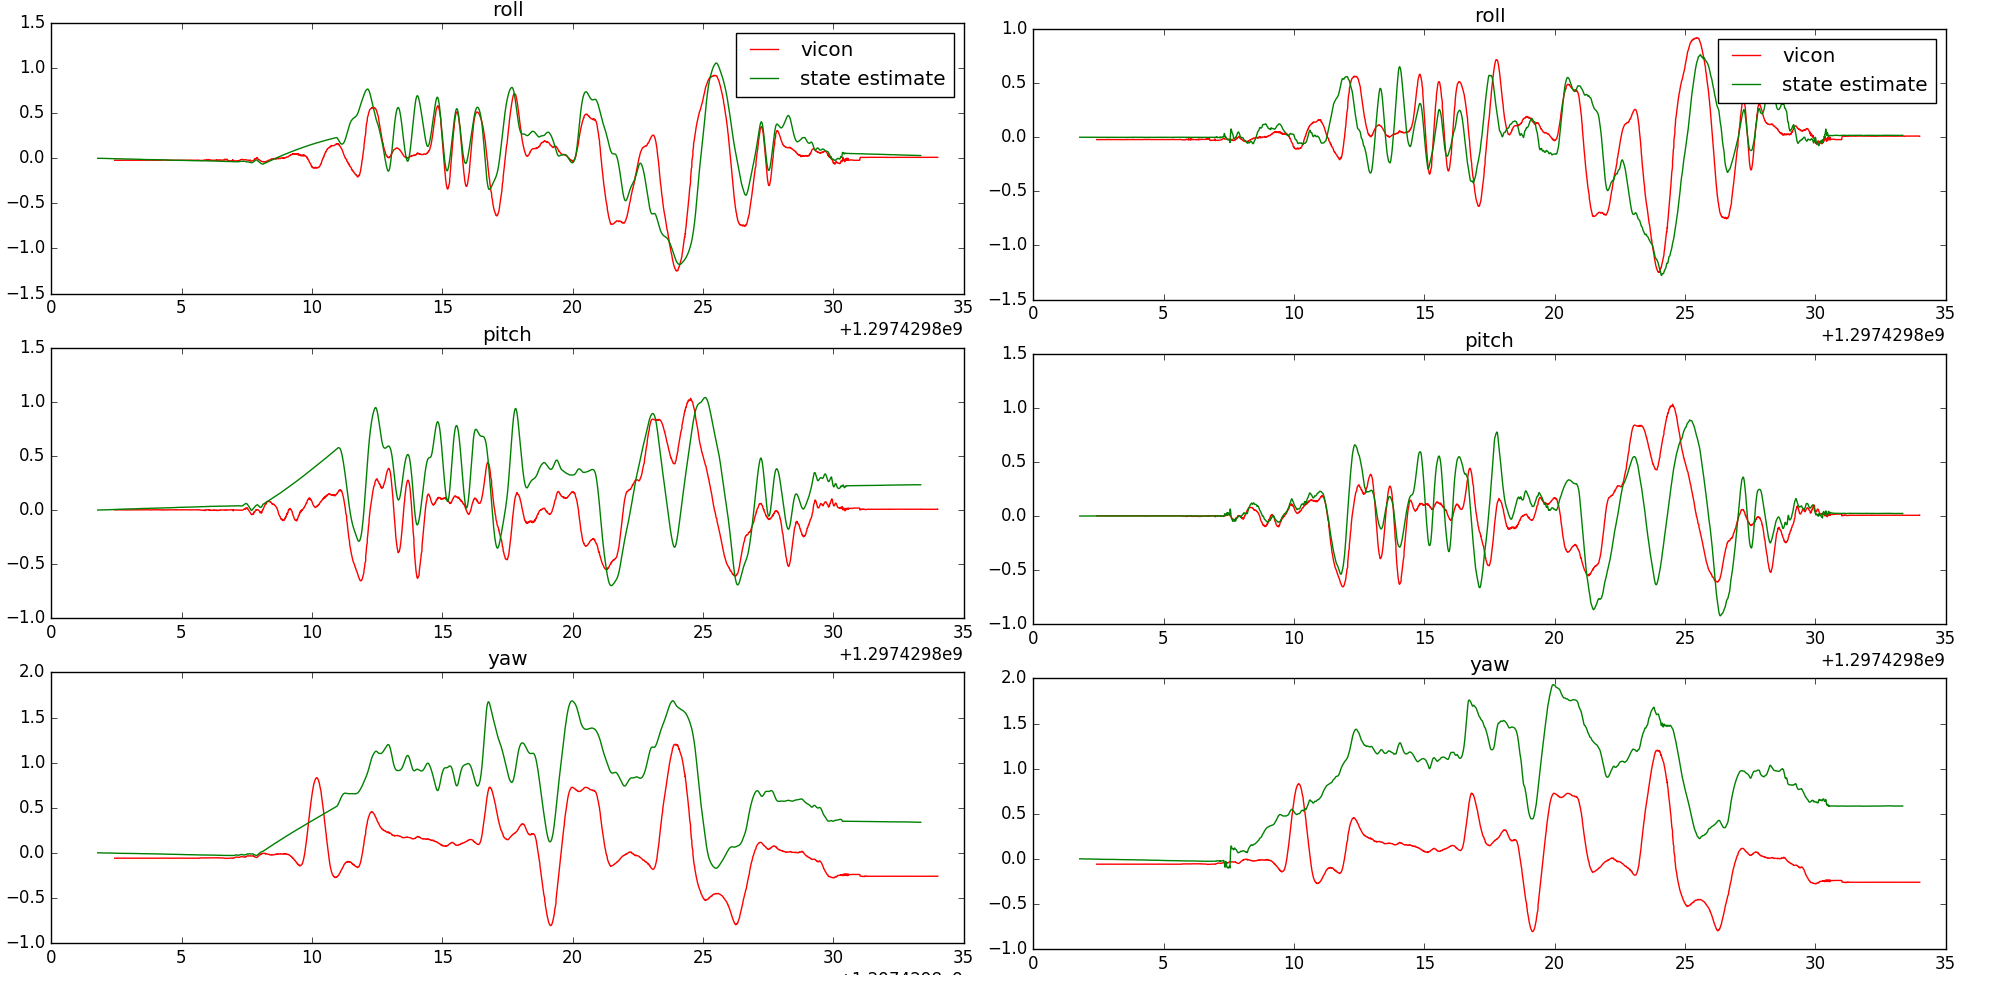
\includegraphics[width=\textwidth,height=5cm]{compare4}
  \caption{Left: Prediction only. Right: UKF compared to ground truth (red) (data set 4).}
  \label{compare4}
\end{figure*} 

\begin{figure*}
  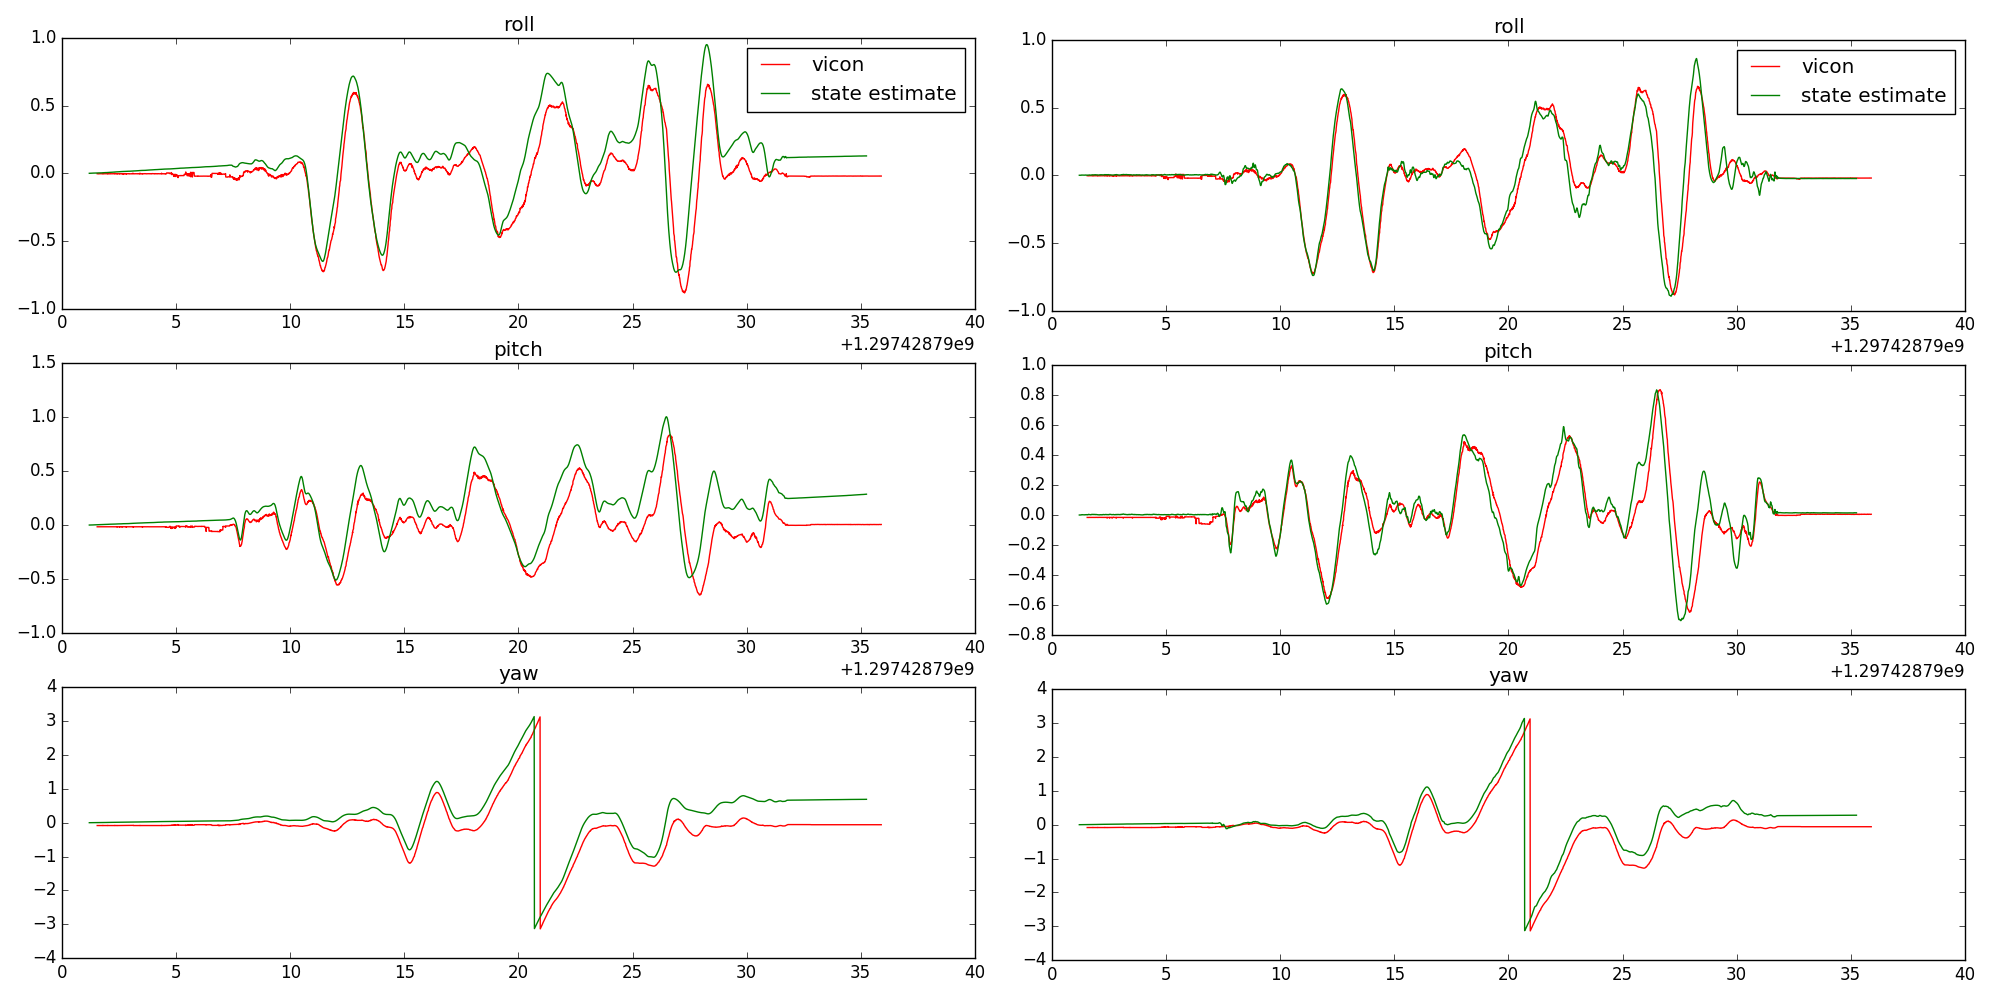
\includegraphics[width=\textwidth,height=5cm]{compare3}
  \caption{Left: Prediction only. Right: UKF compared to ground truth (red) (data set 5).}
  \label{compare5}
\end{figure*}

\begin{figure*}
  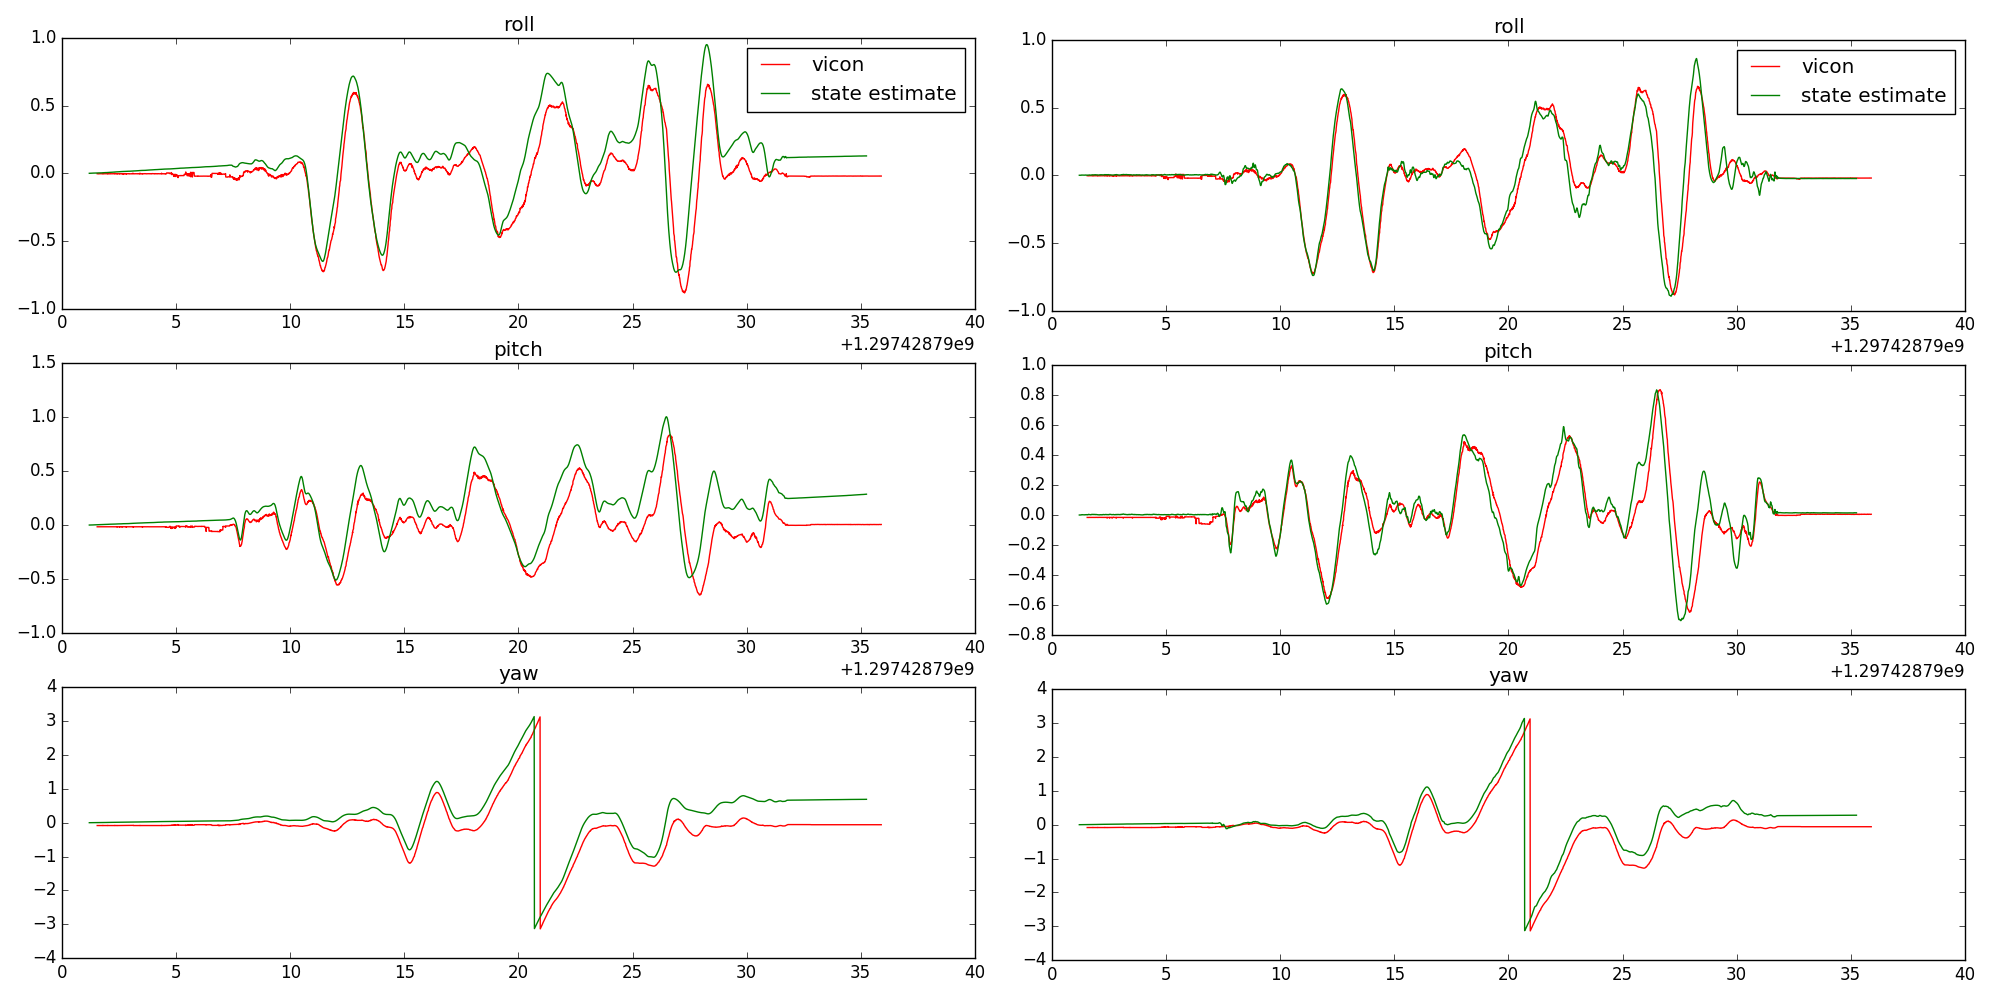
\includegraphics[width=\textwidth,height=5cm]{compare3}
  \caption{Left: Prediction only. Right: UKF compared to ground truth (red) (data set 6).}
  \label{compare6}
\end{figure*} 

\begin{figure*}
  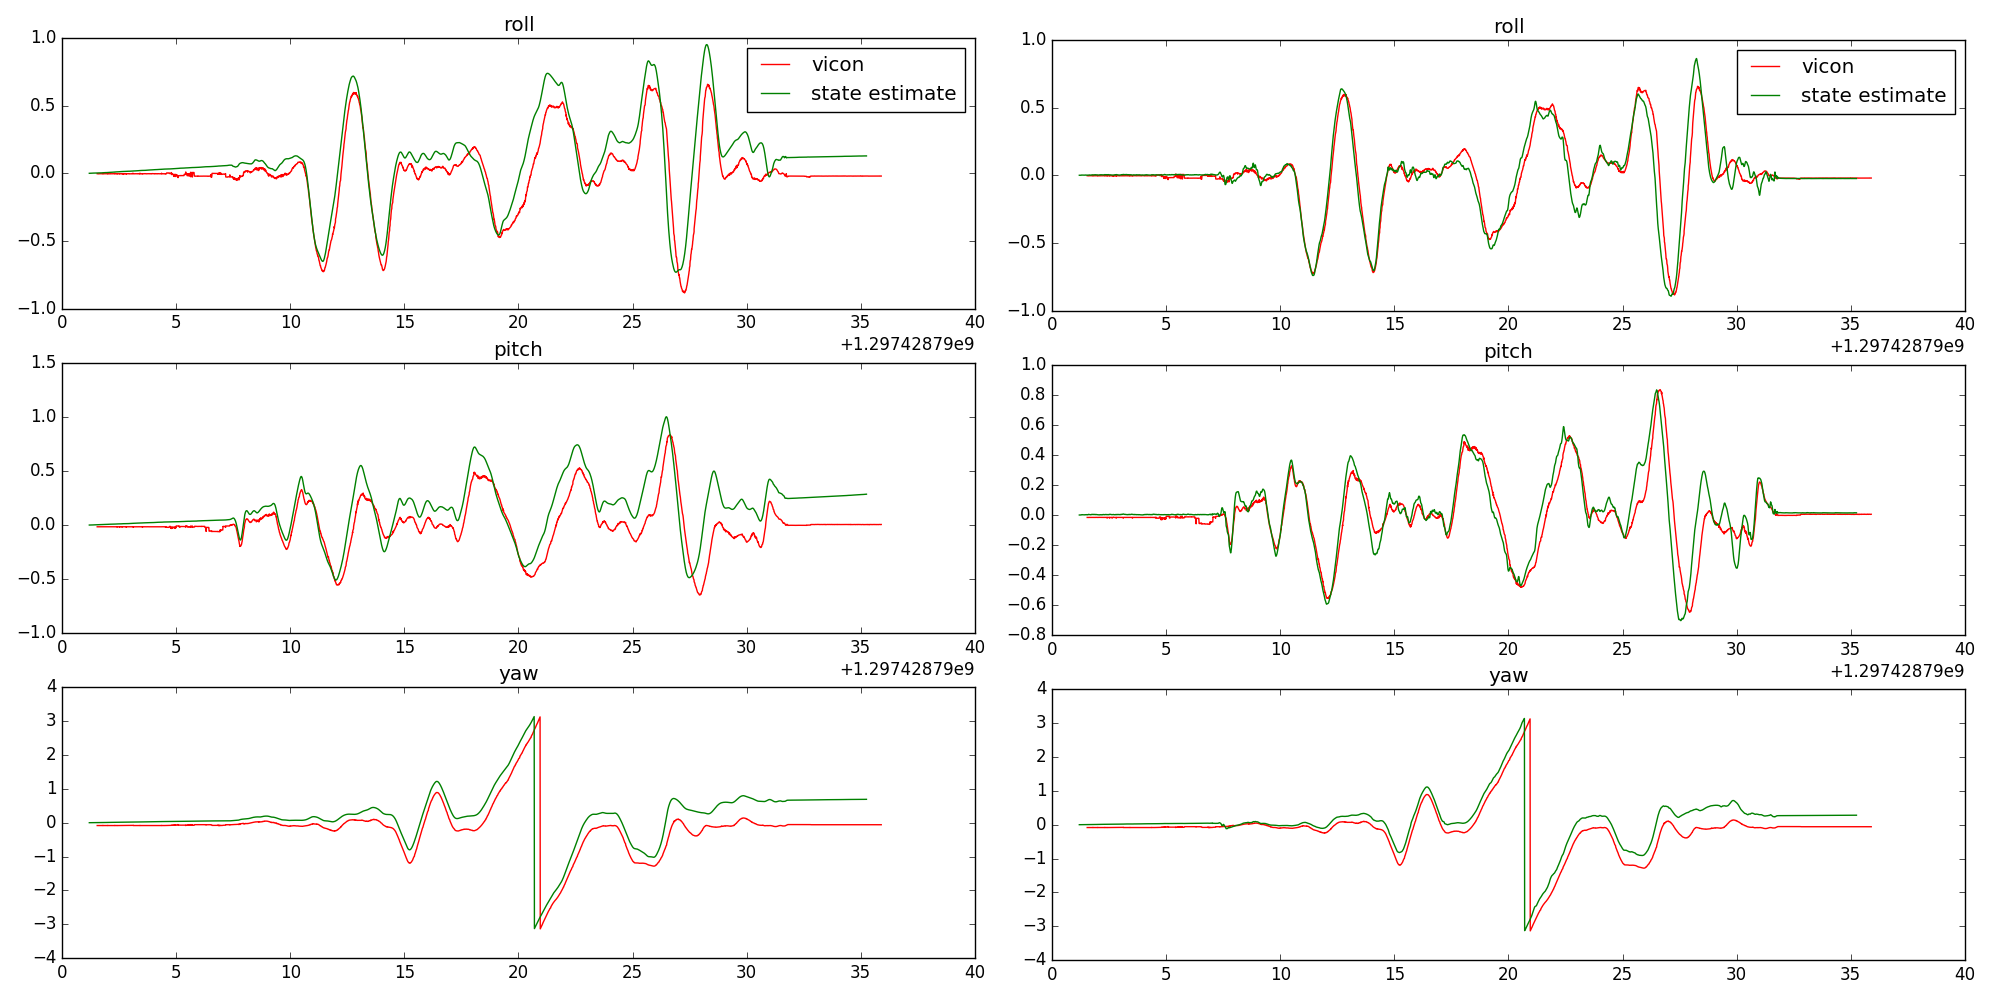
\includegraphics[width=\textwidth,height=5cm]{compare3}
  \caption{Left: Prediction only. Right: UKF compared to ground truth (red) (data set 7).}
  \label{compare7}
\end{figure*}

\begin{figure*}
  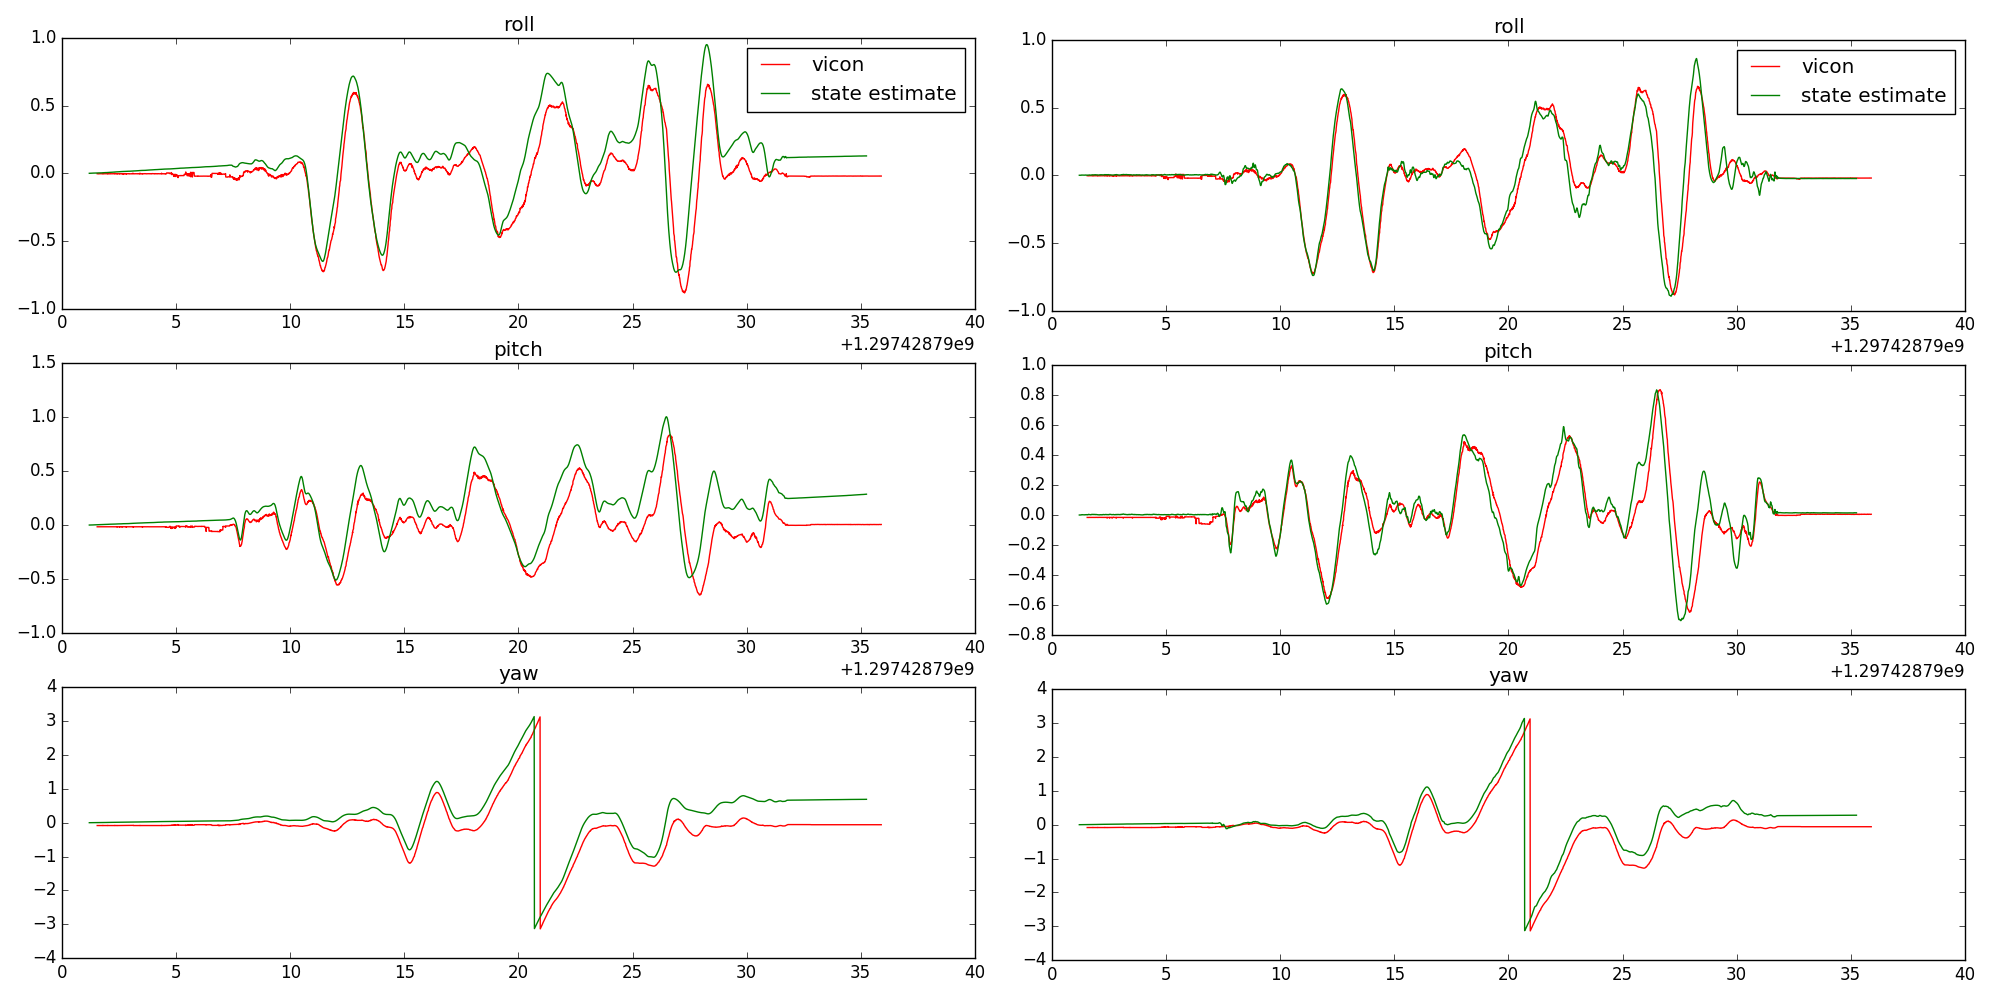
\includegraphics[width=\textwidth,height=5cm]{compare3}
  \caption{Left: Prediction only. Right: UKF compared to ground truth (red) (data set 8).}
  \label{compare8}
\end{figure*}

\begin{figure*}
  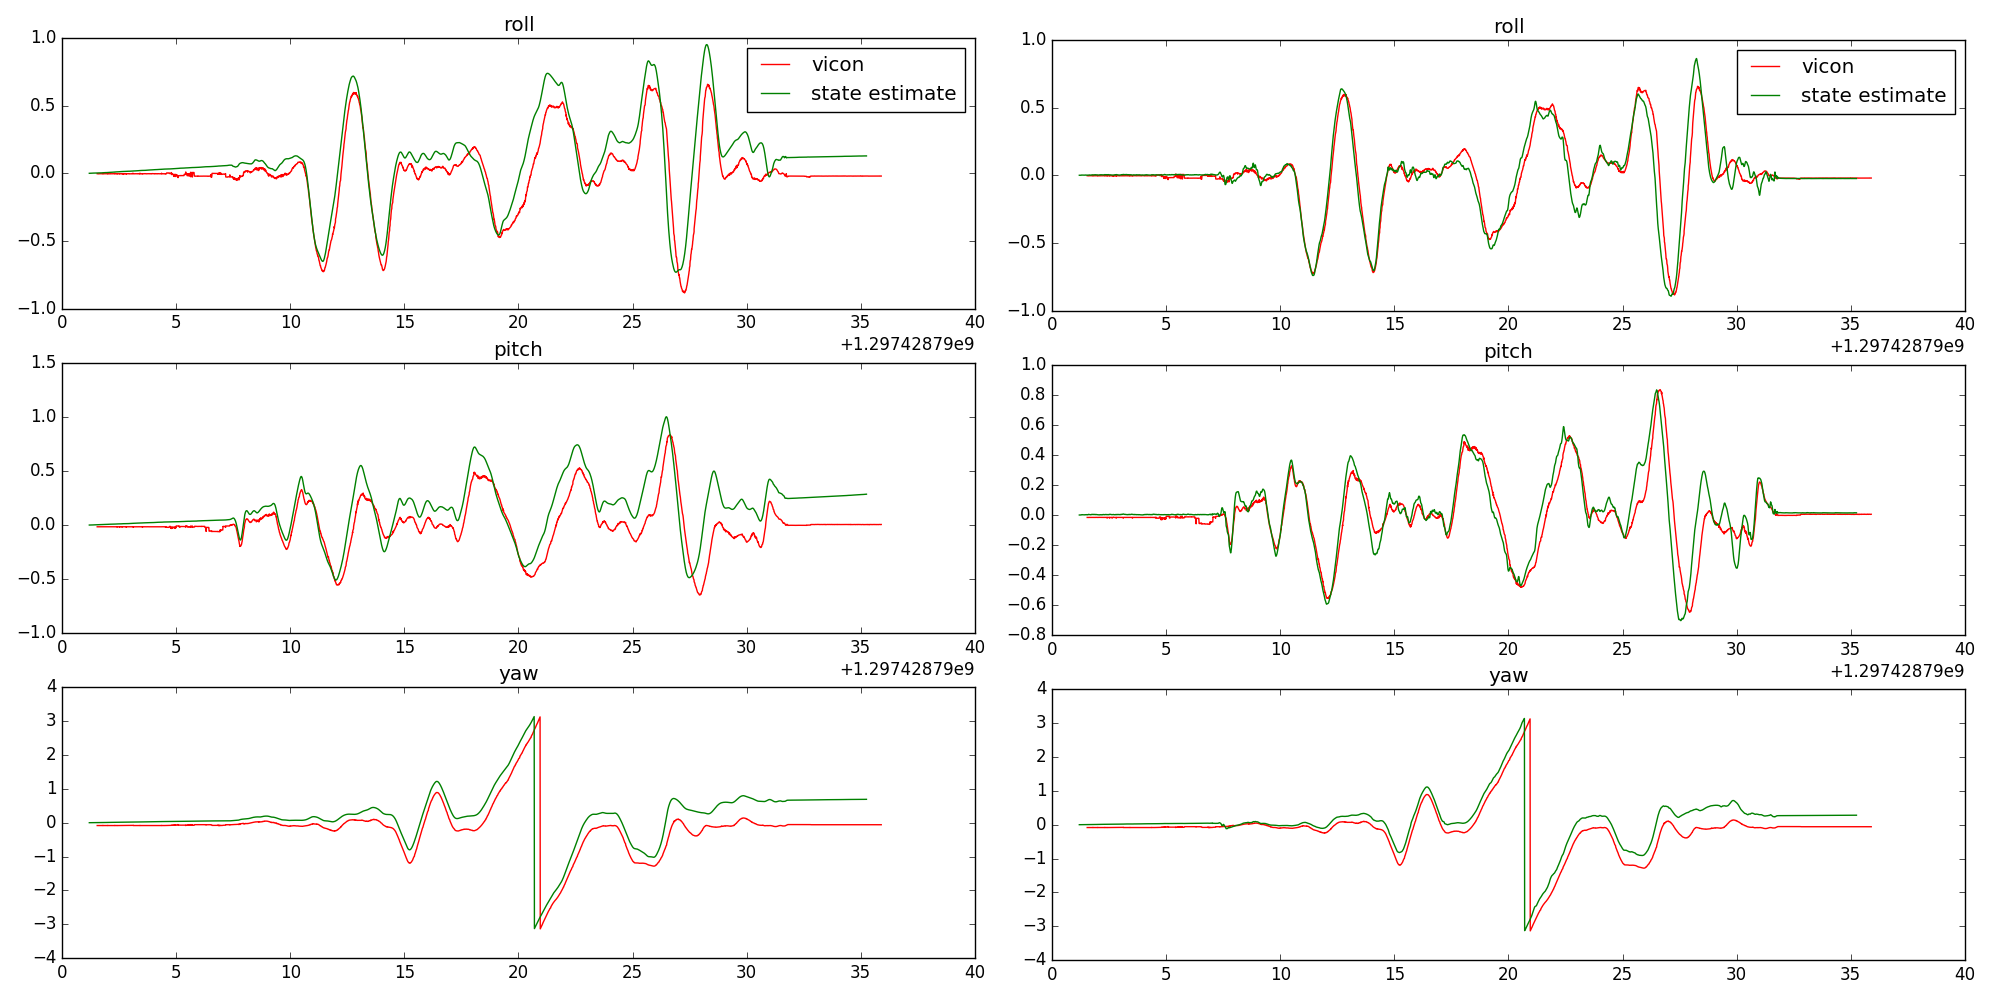
\includegraphics[width=\textwidth,height=5cm]{compare3}
  \caption{Left: Prediction only. Right: UKF compared to ground truth (red) (data set 9).}
  \label{compare9}
\end{figure*}

\begin{figure*}
  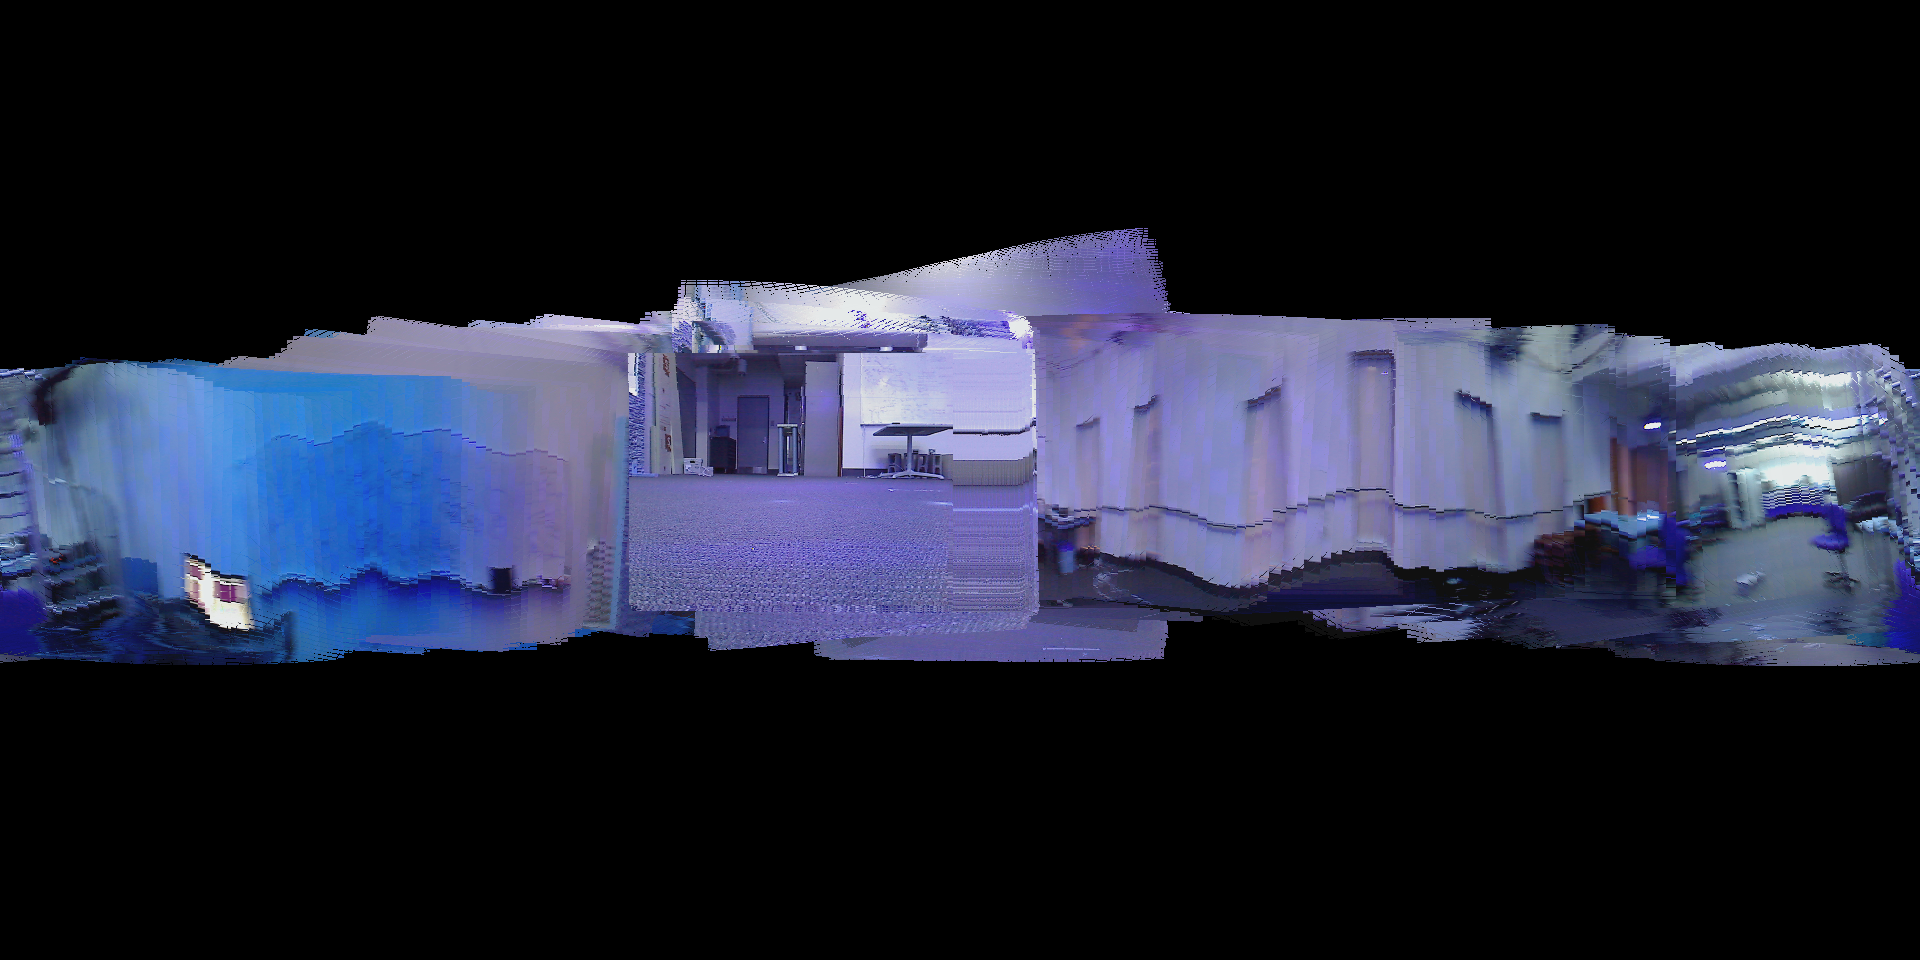
\includegraphics[width=\textwidth,height=10cm]{panorama8}
  \caption{Panorama generated from the UKF (data set 8).}
  \label{panorama8}
\end{figure*}

Results on the test set are show in \ref{test10} - \ref{test13} with respective panoramas in \ref{pano10} - \ref{pano13}. Fewer images were generated in these sets so that the different stitches are clearly seen. Images that are stitched near the top of the panorama display black dots. These are due to the stretching of the images when indexing the panorama. These can potentially be fixed using smoothing and filling or using opening and closing operations. From these sets we can see that the filtering is not optimal. However, the panoramas give a better idea of the device's environment when looking at the video generated in the code as the latest stitch is overwrites previous images. 

   \begin{figure}[thpb]
      \centering
      \framebox{\parbox{3in}{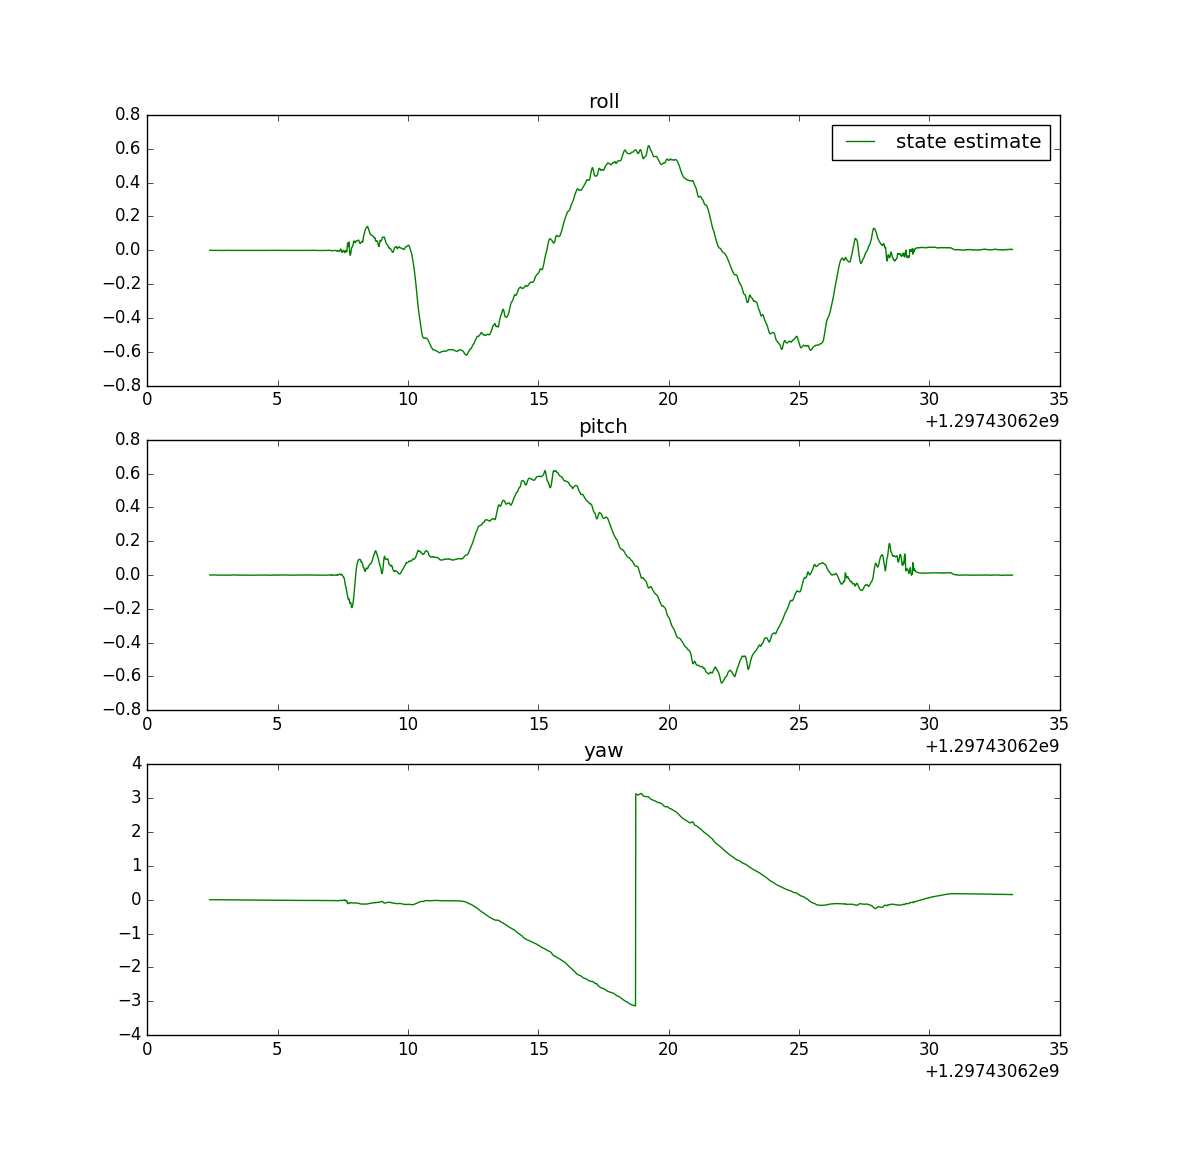
\includegraphics[scale=0.28]{test10}}}
      
      \caption{Result of the filtering on data set 10.}
      \label{test10}
   \end{figure}
   
   \begin{figure}[thpb]
      \centering
      \framebox{\parbox{3in}{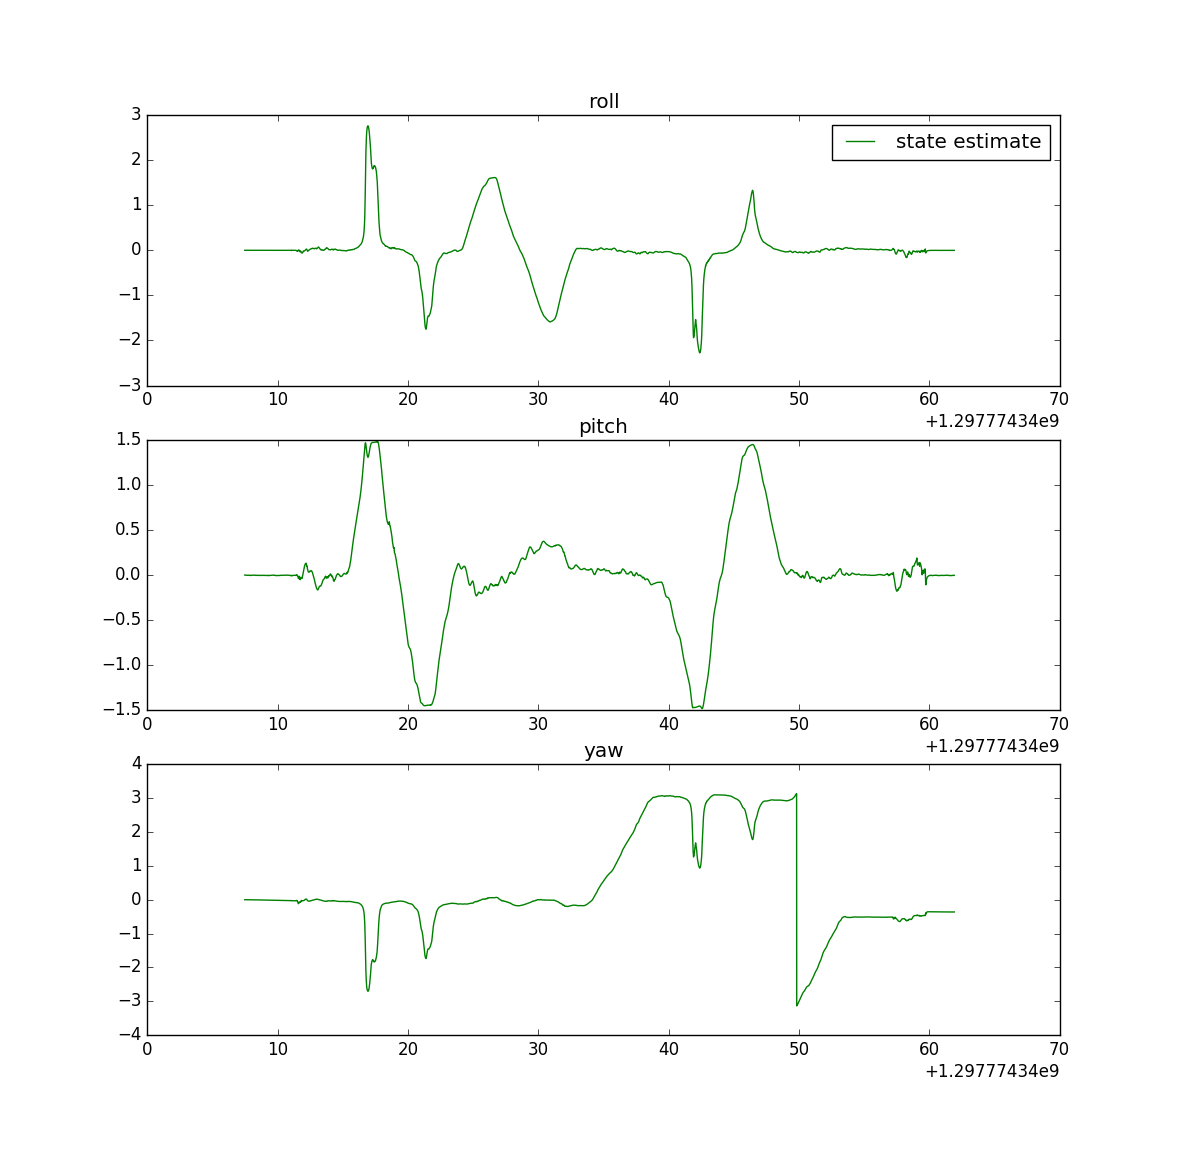
\includegraphics[scale=0.28]{test11}}}
      
      \caption{Result of the filtering on data set 11.}
      \label{test11}
   \end{figure}
   
   \begin{figure}[thpb]
      \centering
      \framebox{\parbox{3in}{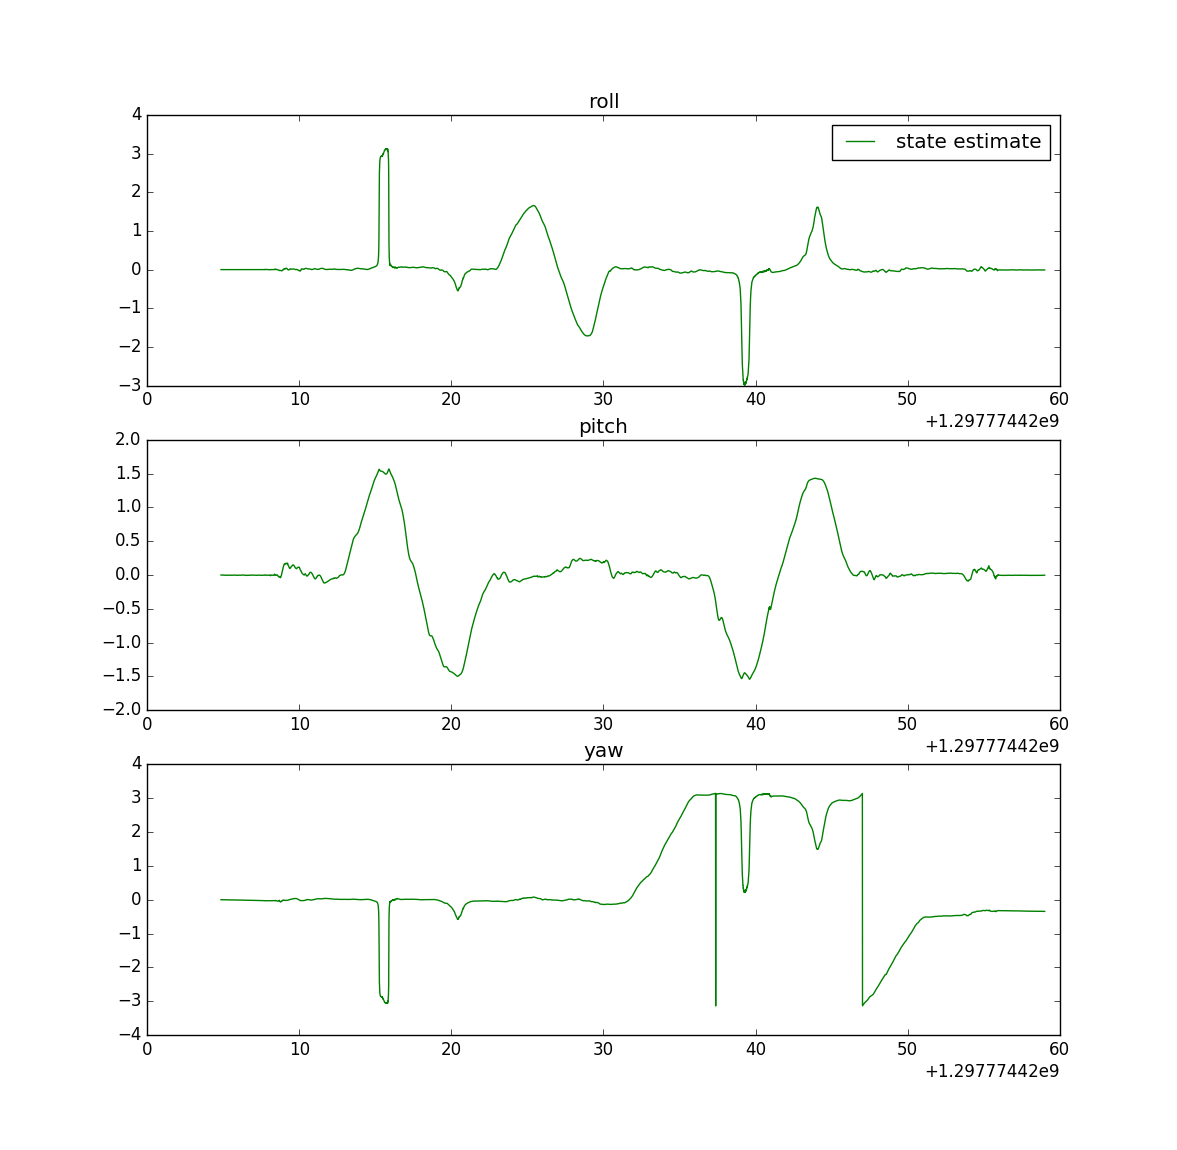
\includegraphics[scale=0.28]{test12}}}
      
      \caption{Result of the filtering on data set 12.}
      \label{test12}
   \end{figure}
   
   \begin{figure}[thpb]
      \centering
      \framebox{\parbox{3in}{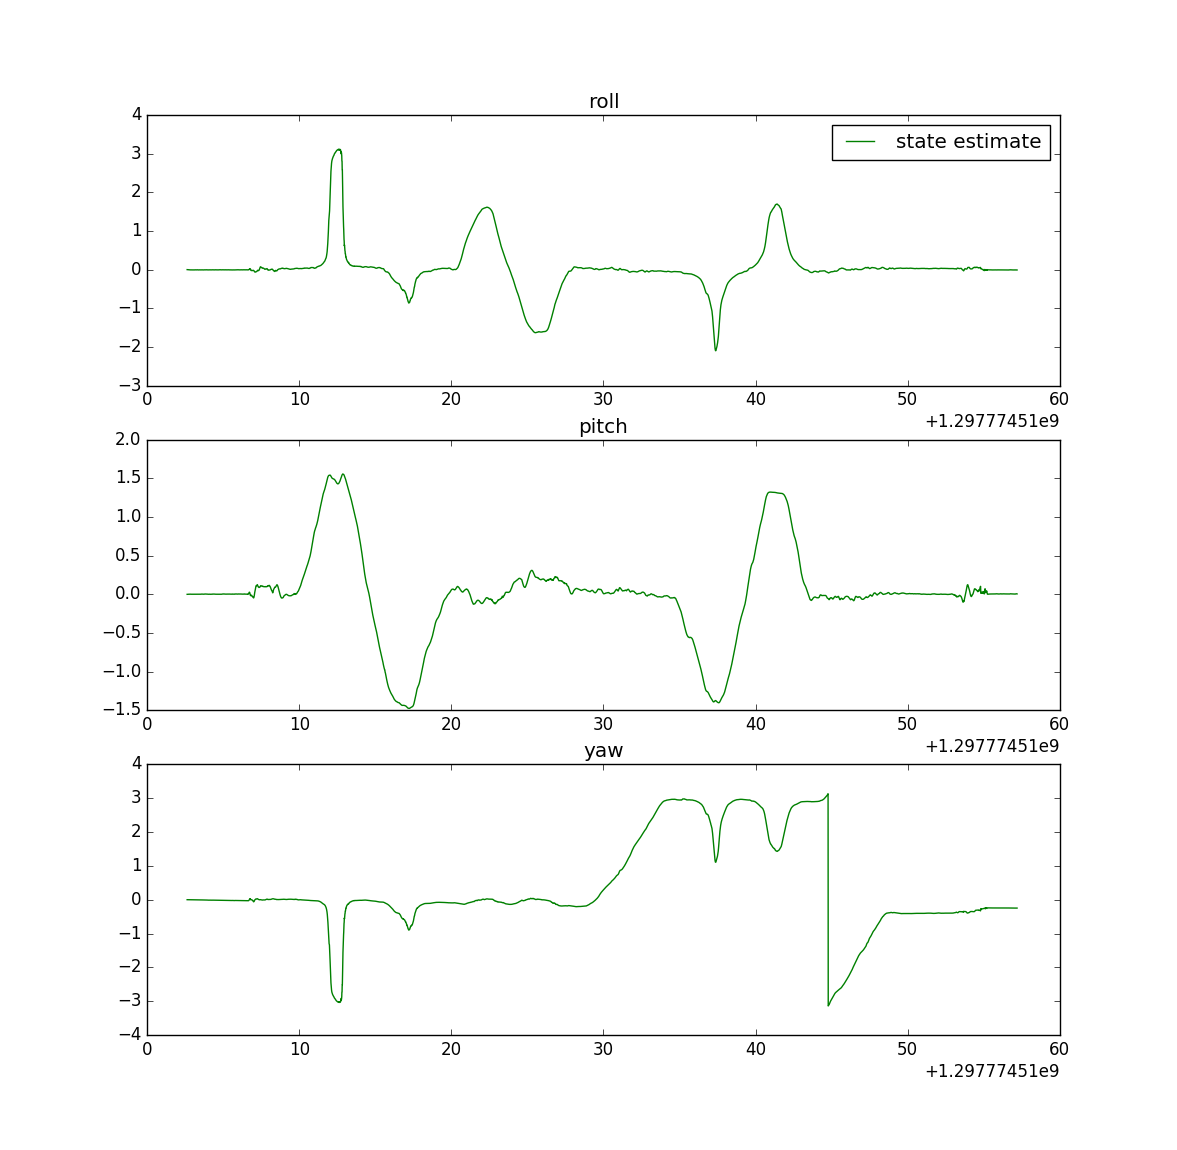
\includegraphics[scale=0.28]{test13}}}
      
      \caption{Result of the filtering on data set 13.}
      \label{test13}
   \end{figure}
   
\begin{figure*} [ht]
  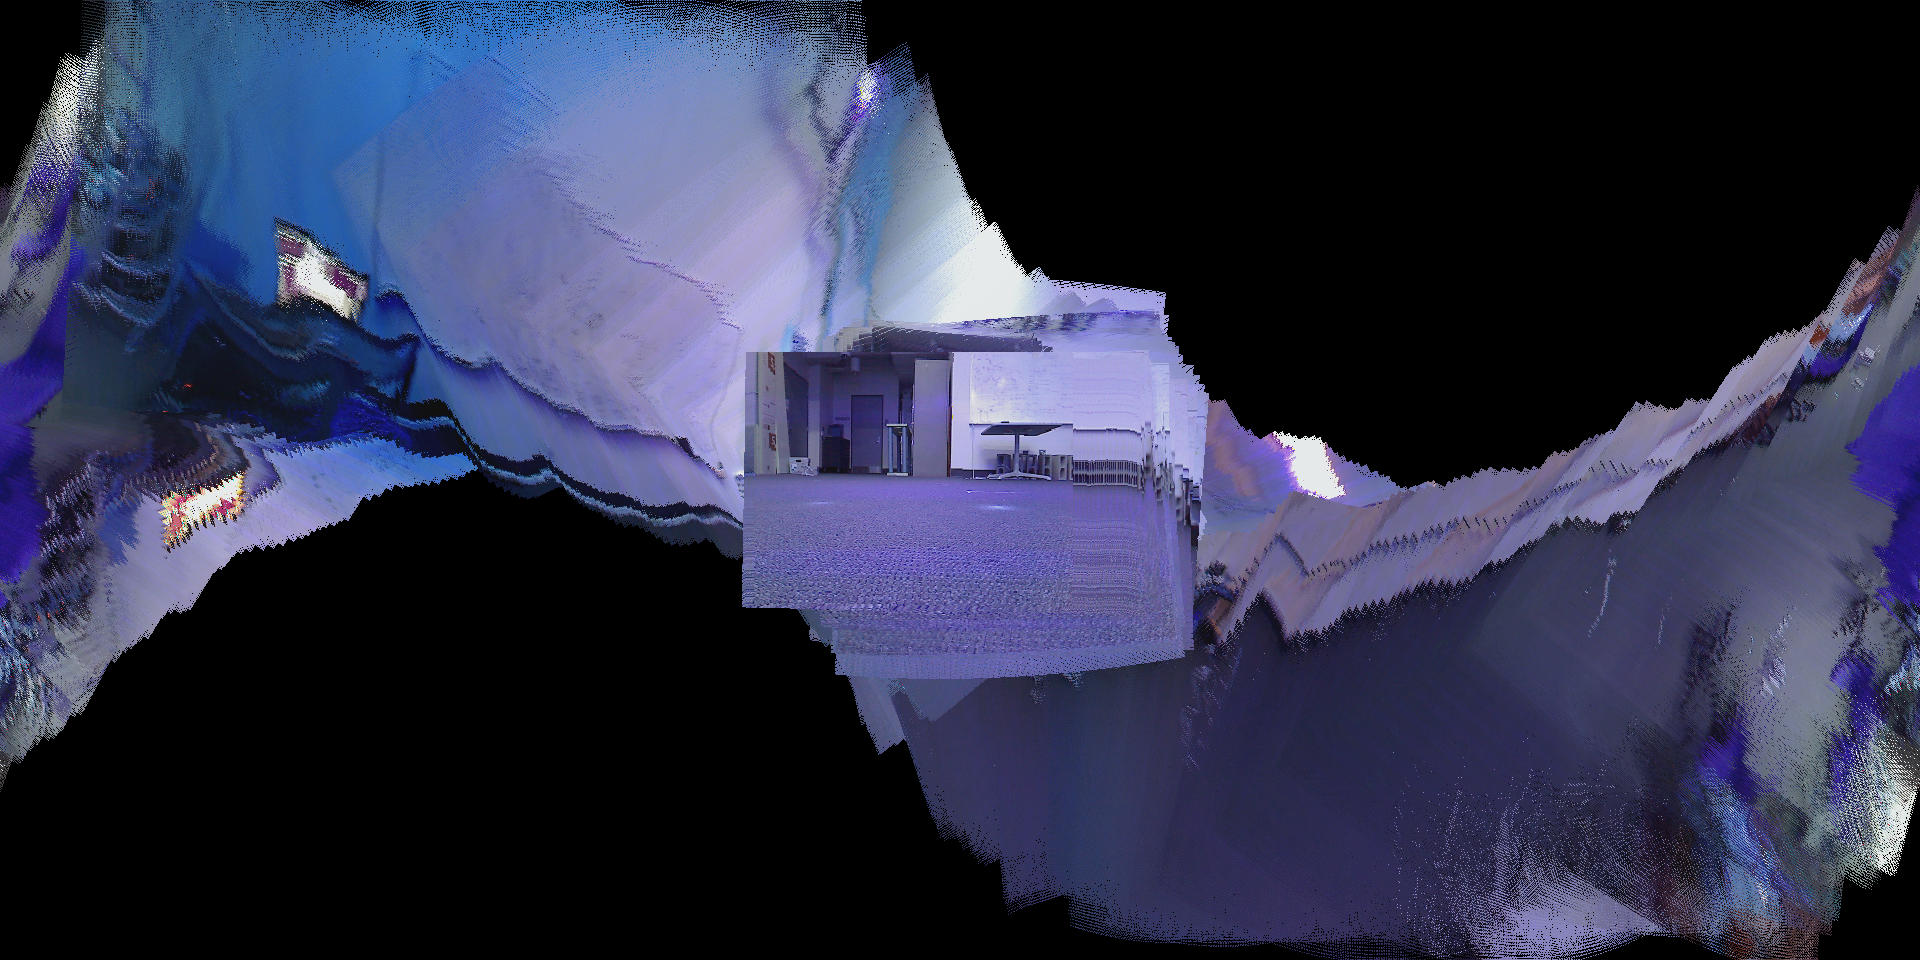
\includegraphics[width=\textwidth,height=5cm]{panorama10}
  \caption{Panorama generated by filtered data (data set 10).}
  \label{pano10}
\end{figure*}

\begin{figure*} [ht]
  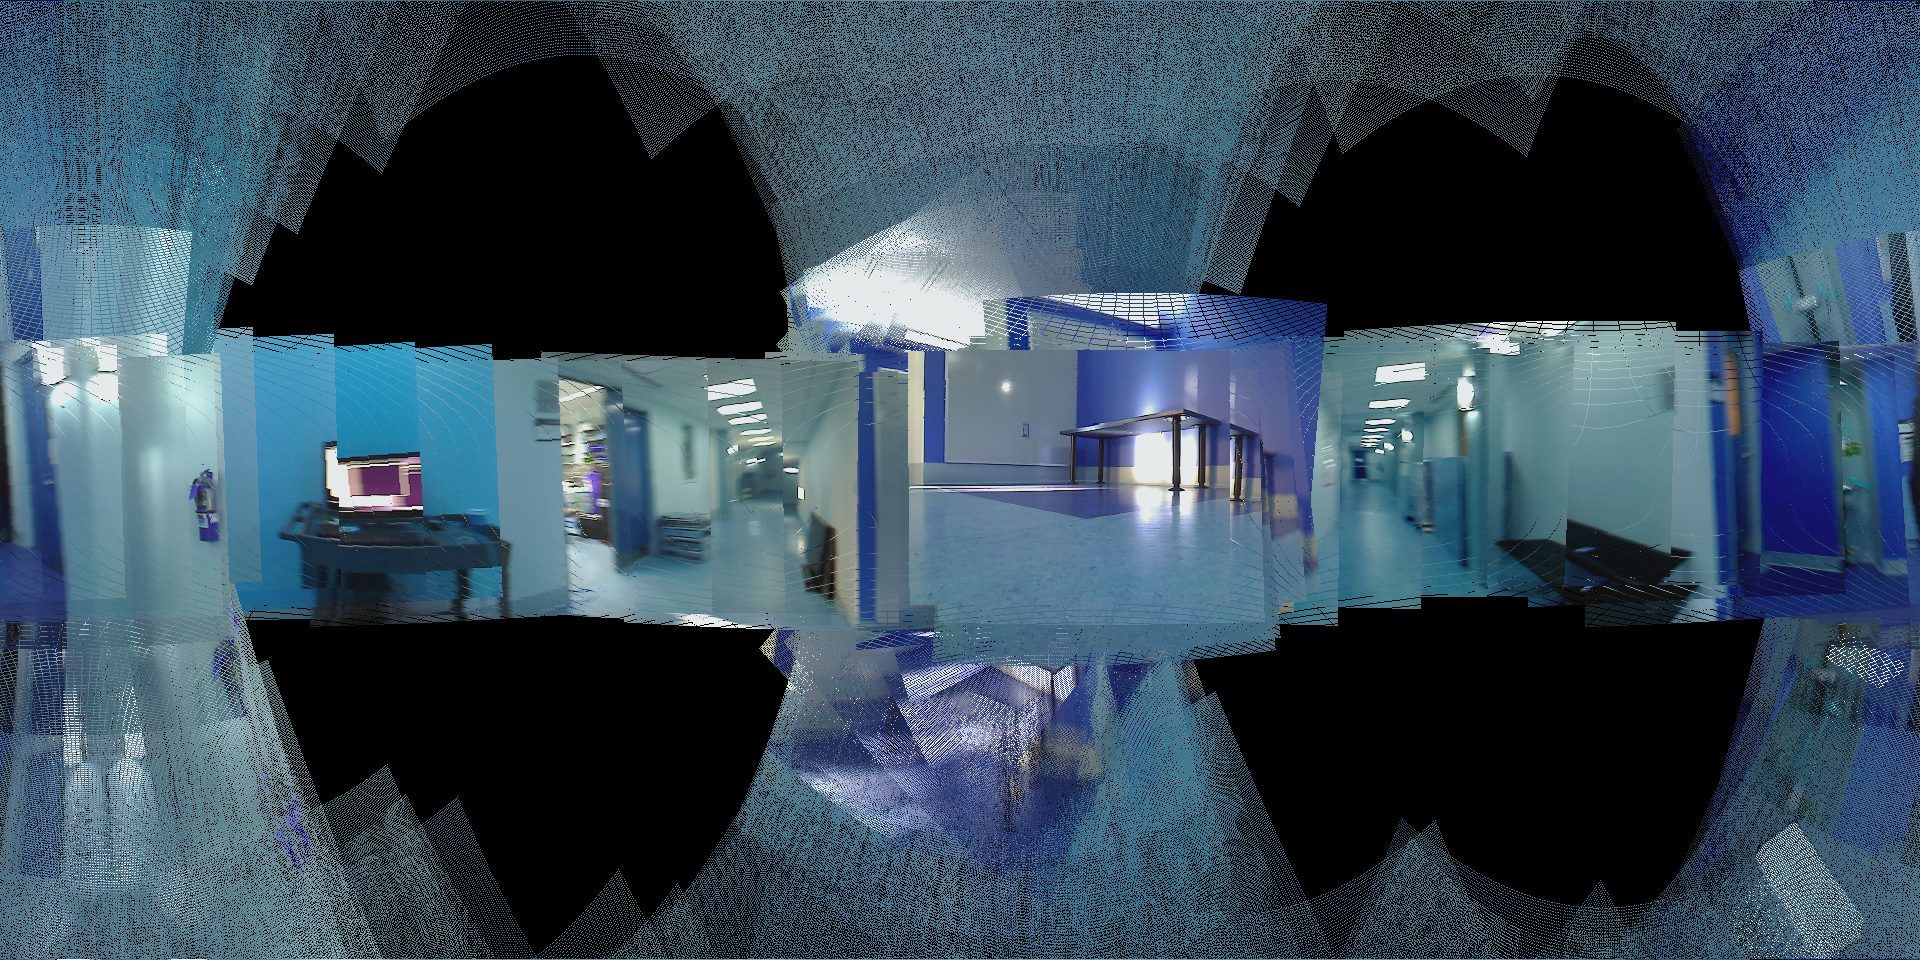
\includegraphics[width=\textwidth,height=5cm]{panorama11}
  \caption{Panorama generated by filtered data (data set 11).}
  \label{pano11}
\end{figure*} 

\begin{figure*} [ht]
  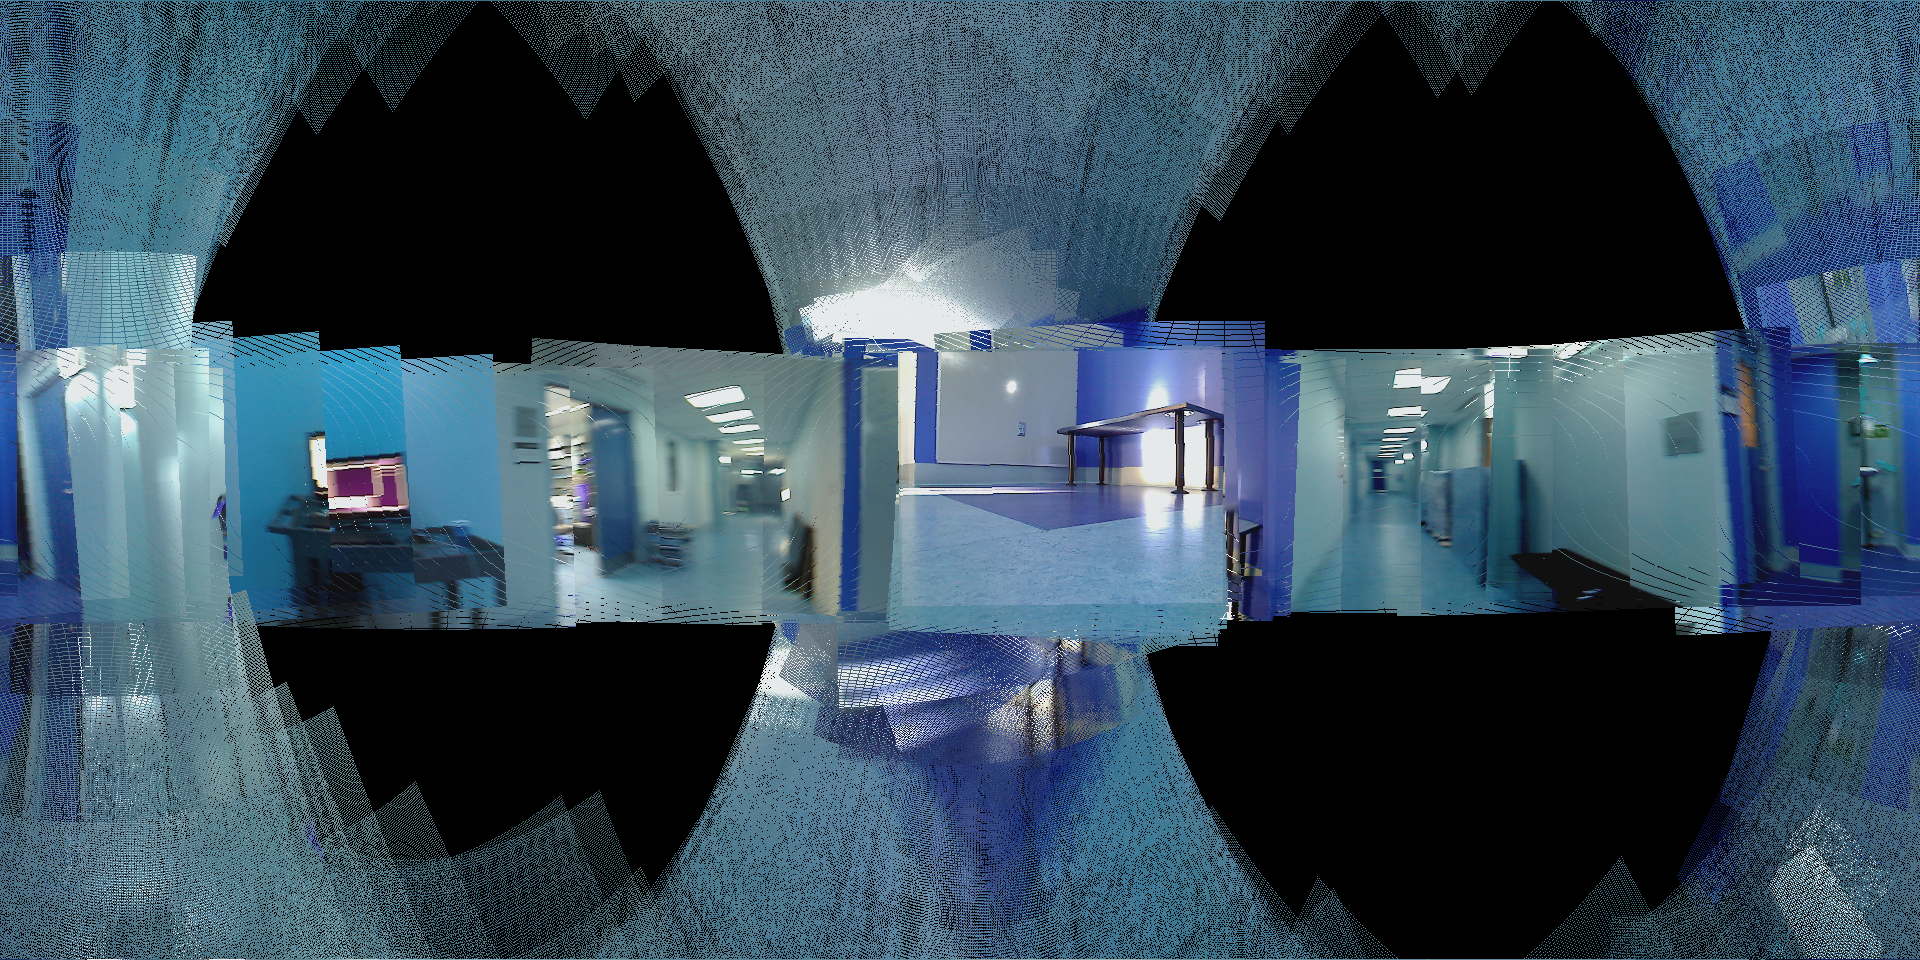
\includegraphics[width=\textwidth,height=5cm]{panorama12}
  \caption{Panorama generated by filtered data (data set 12).}
  \label{pano12}
\end{figure*}

\begin{figure*} [ht]
  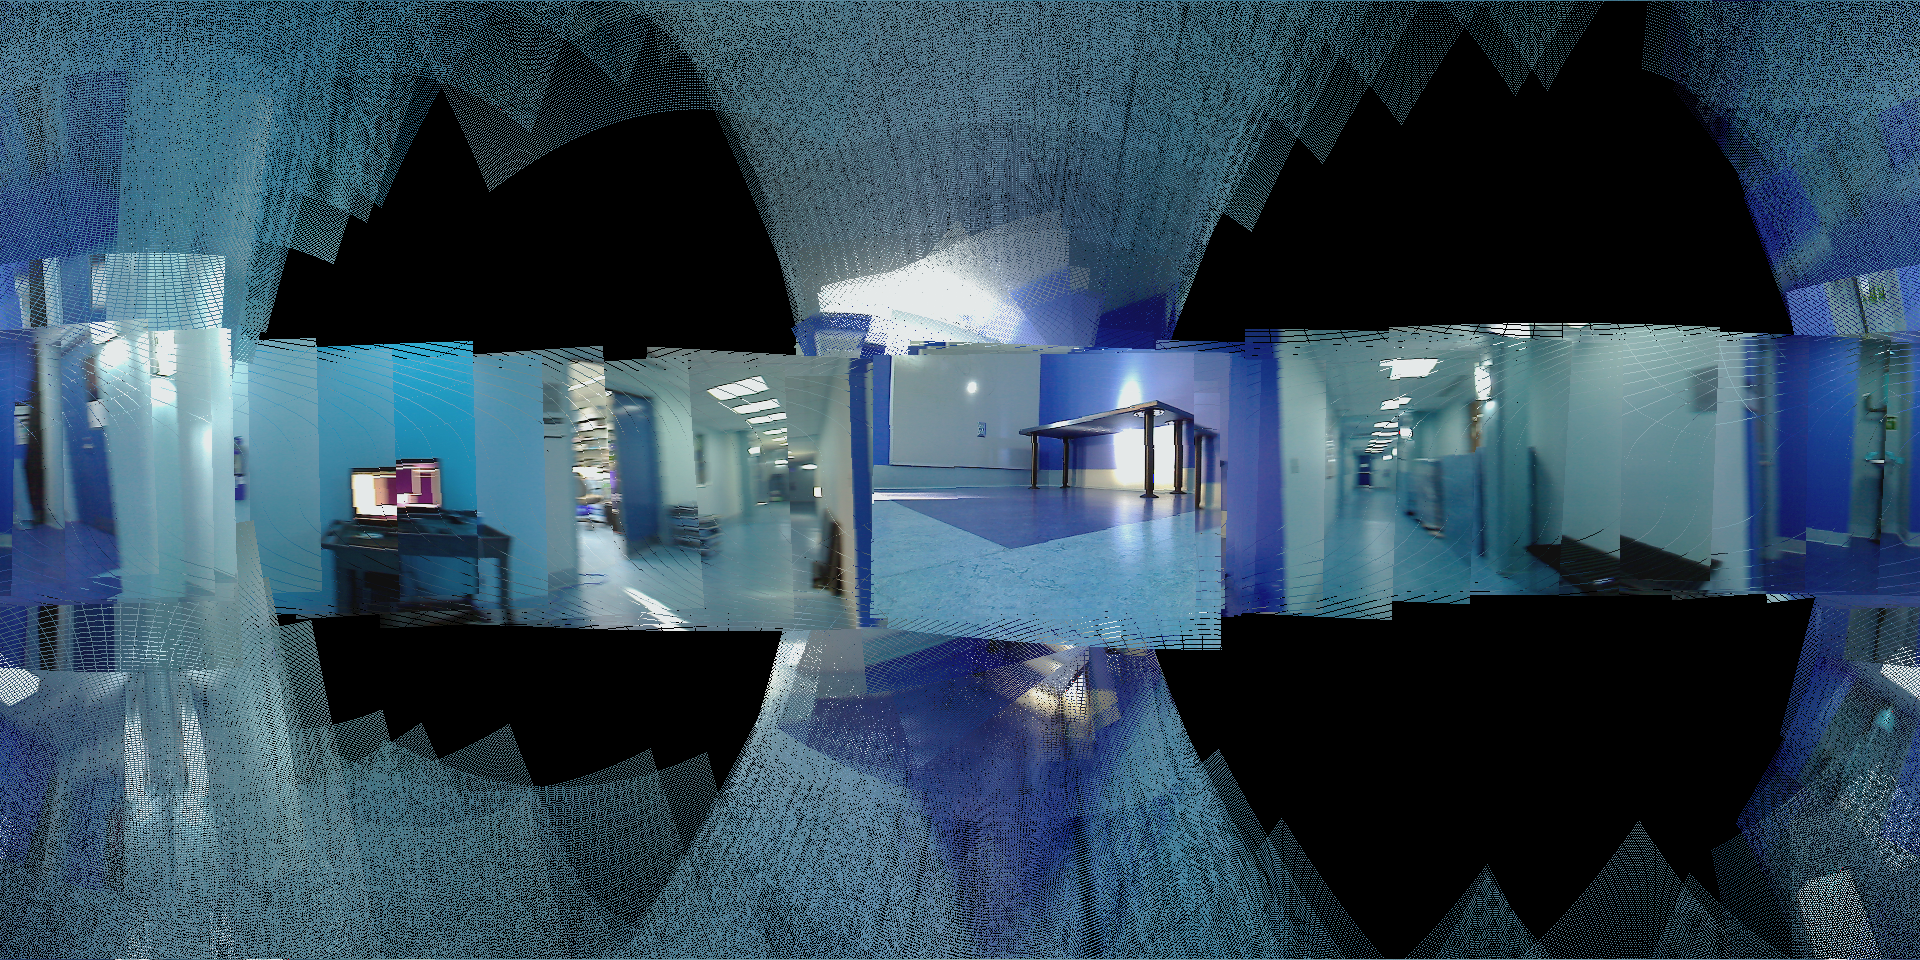
\includegraphics[width=\textwidth,height=5cm]{panorama13}
  \caption{Panorama generated by filtered data (data set 13).}
  \label{pano13}
\end{figure*} 

\section{DISCUSSION}
An Unscented Kalman Filter was implemented that combining measurements from an IMU for orientation estimation. The filter performed better than prediction using gyroscopic values or acceleration values alone. A panoramic stitching methodology based on filter orientation was implemented and provided a good foundation for further image processing to create a map of the robot's environment.

Speed improvements are possible by further vectorizing and minimizing occurence of repeated calculations.

\addtolength{\textheight}{-5cm}   % This command serves to balance the column lengths
                                  % on the last page of the document manually. It shortens
                                  % the textheight of the last page by a suitable amount.
                                  % This command does not take effect until the next page
                                  % so it should come on the page before the last. Make
                                  % sure that you do not shorten the textheight too much.

%%%%%%%%%%%%%%%%%%%%%%%%%%%%%%%%%%%%%%%%%%%%%%%%%%%%%%%%%%%%%%%%%%%%%%%%%%%%%%%%

\begin{thebibliography}{99}

\bibitem{c1} E. Kraft, ÒA Quaternion-based Unscented Kalman Filter for Orientation Tracking.

\end{thebibliography}

%%%%%%%%%%%%%%%%%%%%%%%%%%%%%%%%%%%%%%%%%%%%%%%%%%%%%%%%%%%%%%%%%%%%%%%%%%%%%%%%

\end{document}
